\documentclass[11pt]{article}
\usepackage[margin=1in]{geometry}
\usepackage[T1]{fontenc}
\usepackage[utf8]{inputenc}
\usepackage{lmodern}
\usepackage{amsmath,amssymb,amsthm}
\usepackage{booktabs}
\usepackage{longtable}
\usepackage{array}
\usepackage{enumitem}
\usepackage{xcolor}
\usepackage{tikz}
\usepackage{pgfplots}
\pgfplotsset{compat=1.17}
\usepackage[colorlinks=true,linkcolor=blue!50!black,citecolor=blue!50!black,urlcolor=blue!50!black]{hyperref}

% ---------- notation ----------
\newcommand{\C}{\mathbb{C}}
\newcommand{\R}{\mathbb{R}}
\newcommand{\ip}[2]{\langle #1,#2\rangle}
\newcommand{\abs}[1]{\lvert #1\rvert}
\newcommand{\norm}[1]{\lVert #1\rVert}
\newcommand{\Tz}{\mathcal{T}_0}          % canonical product triple
\newcommand{\To}{\mathcal{T}_1}          % second product triple
\newcommand{\E}{E}                       % energy functional
\newcommand{\cstar}{c_\ast}              % constant 3 sqrt6/(sqrt6+1)^2
\newcommand{\hcube}[1]{#1^{\circ 3}}     % entrywise cube

% ---------- status tags (one per claim) ----------
\newcommand{\st}[1]{\textsc{[#1]}}
\newcommand{\stproved}{\st{proved here}}
\newcommand{\stlean}{\st{Lean-checked, as reported}}
\newcommand{\stcert}{\st{computed, interval-certified}}
\newcommand{\stcomp}{\st{computed}}
\newcommand{\stnum}{\st{numerical only}}
\newcommand{\stcited}{\st{cited}}
\newcommand{\stcond}{\st{conditional}}
\newcommand{\stconj}{\st{conjecture / open}}
\newcommand{\streported}{\st{reported by a team workstream, not re-run}}

% ---------- provenance tags ----------
\newcommand{\event}{\textsc{(event work)}}
\newcommand{\prior}{\textsc{(prior work)}}

\newtheorem{theorem}{Theorem}
\newtheorem{lemma}[theorem]{Lemma}
\newtheorem{proposition}[theorem]{Proposition}
\newtheorem{corollary}[theorem]{Corollary}
\theoremstyle{definition}
\newtheorem{definition}[theorem]{Definition}
\theoremstyle{remark}
\newtheorem{remark}[theorem]{Remark}

\setlength{\parskip}{0.35em}
\setlist{itemsep=0.15em,topsep=0.3em}

\begin{document}

% ======================= 00_front =======================
%%%%%%%%%%%%%%%%%%%%%%%%%%%%%%% TITLE BLOCK BEGIN (removed before LLM review) %%%%%%%%%%%%%%%%%%%%%%%%%%%%%%%
\begin{center}
{\LARGE\bfseries The missing fourth basis in dimension six:\\[2pt] what is verified, how far away it is, and how to see it\par}
\vspace{0.8em}
{\large Ren Jie Tee (University of California, Berkeley)\\
Xinrui \textit{[full name and affiliation: to be completed by the team]}\\
Raymond Fong How (Georgia Institute of Technology)\par}
\vspace{0.5em}
Caltech $\times$ SAIR Mathathon, Round 1, Problem 124 \quad$\cdot$\quad Track: Computation/Applied Mathematics\\
15 November 2026\par
\vspace{0.4em}
{\small
Submission repository (code, certificates, data, this report, slides): \texttt{REPOLINK-PLACEHOLDER}\\
code-and-data commit \texttt{COMMIT-PLACEHOLDER}\\[2pt]
Team Lean and audit repository: \texttt{https://github.com/RaymondFongHow/caltech-mathathon-2026}\\
workstream B baseline \texttt{1033fb082aa0a82ffa4708411370434dc7d9fc23}; workstream C audit
\texttt{4360b1a5bc0211dfd8ebfc6b650c500a29dca384}\par}
\end{center}
%%%%%%%%%%%%%%%%%%%%%%%%%%%%%%% TITLE BLOCK END %%%%%%%%%%%%%%%%%%%%%%%%%%%%%%%

\begin{abstract}
\noindent
Problem 124 asks for the maximum number of mutually unbiased bases (MUBs) in $\C^6$. Three computer-assisted
preprints from 2026 claim that the answer is three. We do not offer a fourth proof. We ask three questions about
the claim: how do we know, by how much, and what would it look like in a laboratory.
\emph{How do we know.} We map what each proof rests on; to our reading none is formally verified end to end.
We rerun the published checkers (a full native rerun reproduces the eight principal output files byte for
byte) and corrupt the saved records on purpose (17 of 26 corruptions are detected). We show by interval arithmetic
that two entries of the 2008 numerical table behind the conjecture are near-misses, not solutions. Toward a proof
a person can read, we characterize the order-six Hadamard matrices whose entrywise cube has rank at most two and
show that degree-four sum-of-squares certificates cannot see the obstruction; one universal step remains open.
\emph{By how much.} For the local qubit--qutrit triple, every pure state has energy $\E\ge0.0385$ (an
interval-verified degree-six certificate; the exact minimum $(4-\sqrt6)/40$ is prior work of Erlwein), and
$\E\ge0.0235$ for the second product triple. We prove an elementary inequality that turns such a one-vector bound
into statements about any fourth \emph{basis}: its bias is at least $0.046$, and it loses at least
$3.3\times10^{-4}$ in the four-basis random-access game. Explicit quadruples do better ($0.030$ and
$2.36\times10^{-4}$), so the best approximate quadruples are not completions of the perfect local triple; for
the bias this also holds for all $16$ triples that contain the standard and Fourier bases.
\emph{In a laboratory.} No pure state can hide from the three local measurements: a chi-square test catches every
state with probability $99\%$ within about $239$ shots per setting (large-sample approximation plus simulation),
where the game needs about $10^{8}$ rounds.
\emph{Dimension ten.} The same certified pipeline shows, conditional on a cited root count, that no four MUBs of
$\C^{10}$ contain the standard and Fourier bases.
Every claim is tagged as proved, Lean-checked, computed, cited, conditional or open, and as event work or prior
work.
\end{abstract}

\subsection*{Reading guide: contributions and their status}

Status tags used throughout: \stproved; \stlean; \stcert; \stcomp; \stnum; \stcited; \stcond; \stconj;
\streported. Provenance tags: \event\ for work done during the 40-hour event, \prior\ for everything else.
The three workstreams of the team are called A, B and C; Section~\ref{sec:event} says who did what and how the
AI tools were used and checked.

\begin{center}
\small
\begin{tabular}{@{}p{0.05\textwidth}p{0.50\textwidth}p{0.24\textwidth}p{0.12\textwidth}@{}}
\toprule
 & Contribution (all event work unless marked) & Status & Section\\
\midrule
1 & Trust map of the three 2026 proofs; mutation test of the saved records ($17/26$ detected); full native rerun
    ($8$ principal files byte-identical; $27{,}188$ root records re-certified) & read; computed; reported by
    workstream C & \ref{sec:trust}, \ref{sec:checks}\\
2 & Cube-rank criterion for order-six Hadamard matrices; cubic norm cap; quartic sum-of-squares obstruction;
    the universal step is open & proved (one cited ingredient); computed; open & \ref{sec:structure}\\
3 & Two entries of the 2008 constellation table are certified near-misses & interval-certified & \ref{sec:const}\\
4 & Energy gap: $\E>1/72$ analytically; $\E\ge0.0385$ and, for the second product triple, $\E\ge0.0235$ by
    certificate. The exact value on the canonical triple is \emph{prior work} \cite{Erlwein} & Lean-checked as
    reported; interval-certified; cited & \ref{sec:gap}\\
5 & Vector-to-basis theorem: any fourth basis has bias $>0.046$ and game loss $>3.3\times10^{-4}$; design lesson
    against explicit quadruples, also for all $16$ triples containing $\{I,F_6\}$ (bias) & proved here, from certified inputs & \ref{sec:bridge}, \ref{sec:sets}\\
6 & Hide and seek: about $239$ shots per setting detect every pure state; the game needs about $10^8$ rounds &
    computed (asymptotic and simulated; not a finite-sample theorem) & \ref{sec:hide}, \ref{sec:game}\\
7 & Dimension ten: no four MUBs contain $\{I,F_{10}\}$ & conditional on a cited root count & \ref{sec:ten}\\
\bottomrule
\end{tabular}
\end{center}

% ======================= s1_question =======================
% ===================== Section 1 =====================
\section{The question}\label{sec:question}

\noindent\emph{Status of this section. This section sets up the problem and the notation. It states known results
(tagged \stcited, \prior), writes out the standard three-basis construction, which we check in one line
(\stproved), and states the three questions the report answers. Nothing in this section is new.}

\paragraph{Mutually unbiased bases.} Two orthonormal bases $\{e_i\}$ and $\{f_j\}$ of $\C^d$ are
\emph{mutually unbiased} (MU) if $\abs{\ip{e_i}{f_j}}^2=1/d$ for all $i,j$. In quantum mechanics an orthonormal
basis is a measurement with $d$ outcomes, and $\abs{\ip{e_i}{\psi}}^2$ is the probability of outcome $i$ on the
state $\psi$ (the Born rule). Two bases are MU exactly when a state that gives a certain outcome in one
measurement gives all $d$ outcomes with equal probability $1/d$ in the other: the two measurements are
\emph{complementary}, like position and momentum. Write $N(d)$ for the largest number of pairwise MU bases of
$\C^d$. One has $N(d)\le d+1$; a full set of $d+1$ MU bases determines an unknown state from outcome statistics
with the smallest statistical error, and $N(d)=d+1$ whenever $d$ is a prime power \cite{WF} \stcited\ \prior. MU
bases are used in quantum key distribution, tomography and entropic uncertainty relations (reviews \cite{DEBZ}
and, for composite dimensions, \cite{MWreview}) \stcited\ \prior.

\paragraph{Six is the first open case.} The smallest dimension that is not a prime power is $d=6$. Here three
MU bases are easy to build, no fourth was ever found, and Zauner conjectured in 1999 that $N(6)=3$
\cite{Zauner} \stcited\ \prior. The natural three come from writing $6=2\times3$, that is, from a qubit
(a two-level system) and a qutrit (a three-level system). Let
\[
 H_2=\tfrac1{\sqrt2}\begin{pmatrix}1&1\\1&-1\end{pmatrix},\qquad
 A_0=I_2,\quad A_1=H_2,\quad A_2=\mathrm{diag}(1,i)\,H_2,
\]
\[
 (F_3)_{jk}=\tfrac1{\sqrt3}\,\omega^{jk},\quad \omega=e^{2\pi i/3},\quad D=\mathrm{diag}(1,\omega,\omega),\qquad
 B_0=I_3,\quad B_1=F_3,\quad B_2=DF_3,
\]
where the columns of each matrix are the basis vectors. The \emph{canonical product triple} $\Tz$ consists of
the three bases of $\C^6=\C^2\otimes\C^3$ given by the columns of $U_r=A_r\otimes B_r$, $r=0,1,2$. Here $A_0,A_1,A_2$
are the eigenbases of the Pauli operators $Z$, $X$, $Y$ of the qubit, and $B_0,B_1,B_2$ are three MU bases of the
qutrit. Because $\abs{\ip{a\otimes b}{a'\otimes b'}}^2=\abs{\ip a{a'}}^2\abs{\ip b{b'}}^2=\tfrac12\cdot\tfrac13$
for vectors from different $r$, the triple $\Tz$ is MU, so $N(6)\ge3$ \stproved\ \prior. (The only entries that
need a computation are those of $F_3^\dagger DF_3$; they are $(1+2\omega)/3$ on the diagonal and
$(2+\omega^2)/3$ off it, both of squared modulus $1/3$.) Every vector of $\Tz$ is a product of a qubit state and
a qutrit state, so each of the three measurements can be carried out by measuring the qubit and the qutrit
separately, with no entangling operation. In this sense $\Tz$ is a \emph{local} triple. By the
classification of McNulty and Weigert there are exactly two MU triples of product bases up to equivalence,
$\Tz$ and a second one $\To$ whose third basis is
$\{\lvert0\rangle_y\otimes DF_3\text{ columns},\ \lvert1\rangle_y\otimes D^2F_3\text{ columns}\}$
\cite[eq.~7.19]{MWreview}, \cite{MW12} \stcited\ \prior; here $\lvert0\rangle_y,\lvert1\rangle_y$ are the columns of $A_2$.
Neither product triple extends to four MU bases \cite{MW12} \stcited\ \prior.

\paragraph{The 2026 proofs, and dimension ten.} Between September and November 2026 three computer-assisted
preprints claimed that no four MU bases exist in $\C^6$, so that $N(6)=3$ \cite{OAI,Jaswal1,CWT}
\stcited\ \prior. Section~\ref{sec:trust} explains what each of them rests on. The next composite dimension
that is not a prime power and has the same shape, $10=2\times5$, is open: three MU bases are known from the
same product construction and no fourth basis has been found or excluded \cite{MWreview} \stcited\ \prior.

\paragraph{Our three questions.} A yes/no theorem proved by a large computation leaves three questions that we
think matter to a mathematician and to a quantum-information scientist.
\begin{enumerate}
\item \emph{How do we know?} What exactly has been verified, by which kind of checker, and what can an outsider
re-check? (Sections~\ref{sec:trust}, \ref{sec:checks} and~\ref{sec:structure}.)
\item \emph{By how much?} ``No fourth basis'' says that a certain distance is positive. How large is it, for
single states and for whole bases? (Sections~\ref{sec:const} and~\ref{sec:number}.)
\item \emph{What would it look like in a laboratory?} If one prepares the best candidate state and measures the
three local bases of $\Tz$, how many repetitions show that it is not unbiased? (Section~\ref{sec:number}.)
\end{enumerate}

\paragraph{Roadmap.} Section~\ref{sec:trust} maps what the three 2026 certificates rest on;
Section~\ref{sec:checks} reports the parts that were re-run. Section~\ref{sec:structure} gives structure results
toward a proof a human can read and names the step that is still open. Section~\ref{sec:const} revisits the 2008
numerical table of partial fourth bases. Section~\ref{sec:number} turns ``no fourth basis'' into numbers: an
energy gap for a fourth vector, a bound for a whole fourth basis, and a detection test with shot counts.
Section~\ref{sec:ten} carries the certified Fourier method to dimension ten, conditionally on a cited root count.
Sections~\ref{sec:support}, \ref{sec:limits} and~\ref{sec:event} give the claim-support table, the limitations,
and the account of event work and AI use.

% ===================== Section 2 =====================
\section{What was proved: a trust map}\label{sec:trust}

\noindent\emph{Status of this section. This section describes other people's proofs, so every result in it is
\prior\ and tagged \stcited. Where we say a document was ``read by us'', we read it during the event; reading is
not verification, and we did not re-check any of the mathematics described here. The only event work is the
reading and the comparison itself.}

\paragraph{What kind of proof these are.} All three 2026 proofs are proofs by exhaustive cases. After a unitary
change of coordinates, any four MU bases can be taken to start with the standard basis $I$ and a basis
$H/\sqrt6$, where $H$ is a \emph{complex Hadamard matrix} (all entries of modulus one, $HH^\dagger=6I$). The
proofs cut the space of such $H$ (up to symmetries) into finitely many small regions. For each region they
cover the vectors unbiased to both $I$ and $H/\sqrt6$ by small balls, build a graph whose edges record which
pairs of balls could still be orthogonal and which could still be unbiased, and show by a graph search that
two further bases cannot be formed. Each step is an inequality evaluated with controlled rounding error.
This is deductive, not a numerical experiment, but it places trust in programs, compilers and arithmetic
\cite{OAI,Jaswal1,CWT} \stcited\ \prior. Earlier numerical work, such as the finding that the best four bases
reach about $0.9983$ on a scale where $1$ means MU \cite{RLE} \stcited\ \prior, is evidence of a different kind:
a search can miss a configuration (Section~\ref{sec:const} gives an instance).

Table~\ref{tab:trust} compares the three certificates. Its entries are \stcited\ \prior.

\begin{table}[htbp]
\centering\small
\begin{tabular}{@{}p{0.13\textwidth}p{0.26\textwidth}p{0.25\textwidth}p{0.28\textwidth}@{}}
\toprule
 & OpenAI \cite{OAI,OAIF} & Jaswal \cite{Jaswal1,Jaswal2} & C\'ardenes Wuttig and Tindall \cite{CWT}\\
\midrule
Date & 24 Sep 2026; the proof rests on a run of 4 Oct 2026 & 13 Oct 2026 (v2 21 Oct); triples paper Nov 2026 & 4 Nov 2026 \\
Cover & 249{,}878 seed centers in nine phases, refined in stages A and B & the same method, re-implemented & 2{,}775 balls in four phases plus one ball at the Fourier matrix, after proving the space of non-Tao Hadamard matrices connected\\
Local test & vectors unbiased to both bases covered by small balls; a graph search excludes two further bases (stage C) & the same & the same test with every inequality re-proved, for the direct proof; a second route classifies all MU triples and cites \cite{JMMSW}\\
Arithmetic & IEEE binary64 with safety margins & binary64 intervals with outward rounding & ball arithmetic (Arb) and an independent Julia checker; a few plain floating-point comparisons with margin $10^{-7}$ against an error bound $2\times10^{-9}$\\
Stated conditions & binary64, round-to-nearest, no contraction or fast-math, a specific lowering of \texttt{pow} & processor, compiler and C library implement IEEE arithmetic correctly (``Assumption A'') & correctness of the certifiers; the floating-point model of the rounding note\\
Formal (Lean) status & the Lean development proves $N(6)\le5$ only; the reduction to $3$ rests on computation outside Lean; nothing is formal end to end & none; the author states that no person has read the code & Lean proves ``the atlas certificate implies no four MU bases''; the certificate's numbers are checked outside Lean; the triple classification is not in Lean and has a single checker\\
Read by us & repository index, Lean scope note, preprint Sections 1, 7, 8 and App.~A.1, saved-run instructions, pinned scope and comparator files & AI-prepared summaries only, not checked by us & \texttt{PROOF.md}, \texttt{VERIFY.md}, the rounding note \texttt{ROUNDING.md}, parts of the paper\\
\bottomrule
\end{tabular}
\caption{What each of the three 2026 certificates rests on \stcited\ \prior. ``Read by us'' lists the documents
read during the event; reading is not verification. The OpenAI documents were read at the pinned public revision
\texttt{4eaee87548250b2682affda7d05d947c05554bae} of \texttt{github.com/openai/math}.}\label{tab:trust}
\end{table}

\paragraph{The Lean status of the OpenAI proof, stated cautiously.} The OpenAI release contains a Lean scope
document for its problem and a comparator challenge file. Two of our workstreams read them independently.
Workstream~C reports that the scope document describes a family bound of five and warns that the selected
formal statement does not establish the computer-assisted exclusion of four arbitrary bases; workstream~B
reports that the comparator's displayed conclusion is ``$\mathrm{Attainable}(n)\Rightarrow n\le5$'' and that the
challenge statement in the comparator file ends with \texttt{by sorry}, so that file is not itself a completed
proof artifact \cite{OAIF} \stcited\ \prior. Neither workstream rebuilt the OpenAI Lean project or audited its
axioms. We therefore use the most cautious reading: \emph{the Lean development proves $N(6)\le5$ only; the
reduction to $3$ rests on computation outside Lean; nothing is formal end to end} \stcited\ \prior. The release
also contains a Lean theorem on Fourier vanishing sums (\texttt{OAI.MUB6.fourier\_vanishing}) used as a
supporting lemma; it is not the no-four theorem \cite{OAIF} \stcited\ \prior.

\paragraph{Four gaps between headline and verification.}
\begin{enumerate}
\item \emph{To our knowledge no end-to-end formal proof exists.} Besides the OpenAI status above, the Lean
theorem of \cite{CWT} takes the atlas certificate as a hypothesis, and the external Lean formalization of the
triple classification \cite{YangLean} takes the computer-assisted facts as explicit hypotheses; because they are
hypotheses and not axioms, a ``no extra axioms'' audit does not show them \stcited\ \prior. (The description of
\cite{YangLean} comes from an AI-prepared summary and was not checked by us.)
\item \emph{The proofs share an ancestor.} Jaswal re-implements OpenAI's method. C\'ardenes Wuttig and Tindall use
a different global reduction (a connectedness argument for non-Tao Hadamard matrices) but the same kind of local
test, and state that their proof does not use OpenAI's certificates. All three were produced with substantial AI
assistance, according to their authors \stcited\ \prior.
\item \emph{Floating point remains in the trusted base of all three.} For \cite{CWT} it is confined to a few
comparisons, whose error analysis was corrected once in the repository: the model was extended to cover underflow
and one bound was changed from $10^{-10}$ to $10^{-9}$ \stcited\ \prior.
\item \emph{The problem sheet is out of date.} Its notes say that no independent re-verification of the OpenAI
preprint was found \cite{Sheet}. The preprints \cite{Jaswal1,CWT} are such follow-ups, with the qualifications
above \stcited\ \prior.
\end{enumerate}

% ===================== Section 3 =====================
\section{What an outsider can check}\label{sec:checks}

\noindent\emph{Status of this section. Here we report checks of pieces of the certificates. The proofs being
checked are \prior; the checks are \event. Workstream~A's reruns, mutation test and Fourier redo are \stcomp,
\stcert\ or \stnum\ as marked. Workstream~C's full native rerun was not re-run by the workstream that assembled this
report and is tagged \streported. The sharp phase-ball radius is a complete proof by workstream~C (\stproved). The
section says for each item what was run, at what precision, and what it does and does not establish.}

\subsection{Workstream A: the OpenAI checker, a mutation test, and a partial rebuild}

\paragraph{Checker rerun.} The OpenAI repository contains the saved records of the run of 4 October 2026 (about
80~MB) and a Python program, \texttt{check\_records.py}, that checks them \cite{OAI} \stcited\ \prior. Workstream~A
ran it unmodified under Python~3.13. It exits with status $0$ in about four seconds and reports the counts of the
preprint's Table~1: 249{,}878 seed centers; 764, 774, 757 and 788 stage-A records; 600 and 22{,}379 stage-B records
in 88 batches; 163 unresolved records after the first stage-C pass, 1{,}127 fallback records and none unresolved at
the end; 100 program invocations. The SHA-256 hashes of the eight principal data files agree with the preprint's
Table~2 \stcomp\ \event.

\paragraph{Mutation test.} To learn what the checker's ``pass'' means, workstream~A made copies of the records,
applied 26 small corruptions one at a time, and reran the checker on each copy. This is mutation testing in the
software sense: a corruption that goes unnoticed marks something the checker does not check. The checker detected
17 of the 26 and missed 9 \stcomp\ \event. Table~\ref{tab:mutation} lists them by kind.

\begin{table}[htbp]
\centering\small
\begin{tabular}{@{}p{0.43\textwidth}p{0.09\textwidth}p{0.40\textwidth}@{}}
\toprule
Kind of corruption (number tried) & Detected & Reading\\
\midrule
Record deleted, duplicated or reordered, or file truncated, including three cases where a header or an upstream log was edited to match (8) & 8 of 8 & record counts, log counts and the partition of records into batches are cross-checked\\
Value changed in one of two copies of a record, or in a failure file (2) & 2 of 2 & copies must be byte-identical; failures must be a subsequence of the input\\
Value outside its declared range (3) & 3 of 3 & range checks\\
Exit code, failure file or log altered (3) & 3 of 3 & failed batches must reappear as inputs of the fallback stage\\
Stray file added (1) & 1 of 1 & file membership\\
Record order or failure label changed consistently (2) & 0 of 2 & harmless: neither affects coverage\\
Stored value changed within its range: a phase (also by one unit in the last place), a radius, a certified bound, a seed-center coordinate (6) & 0 of 6 & \textbf{scope gap}: record contents are only range-checked\\
Last-stage record deleted \emph{and} the log counts edited to match (1) & 0 of 1 & \textbf{scope gap}: coverage of a parent ball by its children is not recomputed; the text logs are trusted\\
\midrule
Total (26) & 17 of 26 & \\
\bottomrule
\end{tabular}
\caption{Mutation test of OpenAI's record checker \texttt{check\_records.py}: 26 deliberate corruptions of the saved
records, each applied alone \stcomp\ \event.}\label{tab:mutation}
\end{table}

\paragraph{What the 9 undetected corruptions mean, and what they do not mean.} Two of the nine change nothing that
matters for the proof. The other seven are scope gaps. They show that the checker confirms that the saved files are
internally consistent bookkeeping: accidental loss, truncation or damage is caught, including consistent deletions
at earlier stages, which are caught by downstream counts. The checker does not recompute any inequality, does not
check that the balls cover the parameter space, and does not detect a change of a stored value within its range or
a last-stage deletion made consistently in data and logs \stcomp\ \event. This agrees with the checker's own
documentation of its scope \cite{OAI} \stcited\ \prior. The nine misses are a statement about the checker and
\emph{not} a flaw in the theorem: none of the corruptions came from the real run, and the mathematical content of
the proof rests on rerunning the C++ programs under the stated arithmetic conditions, not on the record checker. A
reader who wants evidence for the theorem must therefore rerun the programs, which is the next step.

\paragraph{Partial rebuild on a second machine.} Workstream~A compiled the published C++ sources with the flags
stated in the preprint (\texttt{g++ -O3 -march=native -ffp-contract=off}) and reran three pieces with the recorded
arguments \stcomp\ \event:
\begin{itemize}
\item the seed cover (\texttt{covrun}): 151{,}744{,}086 pairs checked, 249{,}878 centers, 19 minutes; the output
has the same SHA-256 hash as the saved \texttt{centers.txt};
\item the first of the four shards of stage A: 62{,}470 seed centers, 35 minutes; its 764 records are
byte-identical to the saved \texttt{coarse0.bin};
\item two of the 88 first-pass batches of stage C (numbers 0 and 3): outputs and exit codes identical to the saved
ones, including the two unresolved records of batch 3; a second build with \texttt{-march=x86-64} in place of
\texttt{-march=native} gave the same outputs.
\end{itemize}
Every rerun output was bit-identical to the saved one. The limits: the machine had the same compiler, C library
and operating system as the preprint's (g++ 13.3.0, glibc 2.39, Ubuntu 24.04) and a similar processor (a virtualized
Intel Xeon with AVX-512), so this says little about independence from hardware or compiler; stage B, three quarters
of stage A, 86 of the 88 stage-C batches and the final pass were not rerun by workstream~A; and reproducing outputs
does not check the mathematics that connects them to the theorem.

\subsection{Workstream C: a full native rerun and three worked examples}

\paragraph{Full native rerun.} Workstream~C reran the whole OpenAI pipeline natively: 100 child invocations,
retaining 249{,}878 seed centers, 3{,}083 stage-A records, 600 intermediate and 22{,}379 fine records in 88 batches;
stage C first left 163 unresolved records, the fallback produced 1{,}127 records, and the final unresolved count
was zero. The eight principal output files (\texttt{centers.txt}, the four \texttt{coarse*.bin}, \texttt{mid.bin},
\texttt{fine.bin}, \texttt{fb.bin}) are byte-identical to the released ones. The run used an AMD EPYC x86-64
processor under GNU/Linux with GCC 14.2 and \texttt{-O3 -march=native -ffp-contract=off}, so it differs from the
preprint's environment in compiler version and processor vendor \streported\ \event. In a separate program
(\texttt{src/verify\_roots.py}), workstream~C reconstructed the inverse-like maps of the ``Root'' records (the
records that bound where exact solutions can lie near an approximate center) and checked their inequalities in
128-bit Arb ball arithmetic: it read 27{,}189 records and re-certified 27{,}188 distinct Roots, of which 1{,}143
needed the transposed orientation \streported\ \event. The evidence is at the audit commit
\texttt{4360b1a5bc0211dfd8ebfc6b650c500a29dca384} of the team Lean repository (title block). Both programs and the
original share an AI workflow, so this is not an independent human review; byte agreement does not rule out a
shared source-level error, and it does not prove the analytic covering lemmas \streported\ \event.

\paragraph{Three worked examples.} Workstream~C also wrote out, on small instances, what each kind of certificate
step says \event.
(1) \emph{Region exclusion.} For the qubit vector $\psi_\theta=(\lvert0\rangle+e^{i\theta}\lvert1\rangle)/\sqrt2$ one has
$\abs{\ip{+}{\psi_\theta}}^2=\cos^2(\theta/2)\ge3/4>1/2$ on the whole arc $\abs\theta\le\pi/3$, so no vector in
that arc is unbiased to the $X$ basis \stproved. A certificate excludes every point of a region, endpoints included,
not a sampled point.
(2) \emph{Integer graph test.} A synthetic 12-vertex graph with exactly two disjoint orthogonality 6-cliques and 35
of the 36 required unbiasedness cross edges was run through the unmodified OpenAI stage-C kernel and a separate
subset enumeration: both return ``excluded''; with the 36th edge both return ``possible''; with the search cap set
to zero the kernel returns ``unknown'', which the pipeline must refine and never count as an exclusion
\streported.
(3) \emph{Geometric Root certificate.} Record zero of the released \texttt{coarse0.bin} was decoded; its stored
constants give a normal-displacement bound $n(r)=n_0+\iota r+Cr^2\approx0.0736<37/500$, checked as an exact rational
comparison of the binary64 values \streported. Such a record bounds where exact Hadamard matrices can lie relative to
an approximate center; it does not assert that one exists nearby.

\subsection{A sharp radius for phase balls}

The graph test needs distinct vertex labels: two vectors of two further MU bases are either orthogonal or unbiased,
so they must not lie in the same small ball of phases. The OpenAI source uses the sufficient radius $s<1/10$
\cite{OAI} \stcited\ \prior. Workstream~C found the exact threshold. Write $e(t)=\exp(2\pi it)$ and, for $v\in\R^6$,
\[
 B(v,s)=\Bigl\{\tfrac{\lambda}{\sqrt6}\textstyle\sum_{j=0}^5 e(v_j+x_j)\lvert j\rangle:\ \abs\lambda=1,\ \sum_j x_j=0,\
 \norm{x}_2\le s\Bigr\},
\]
a ball of phase vectors (radius measured in turns, not in Hilbert-space distance).

\begin{proposition}[Sharp phase-ball radius]
Let $s_\ast=\sqrt6\,\arccos(1/\sqrt6)/(4\pi)=0.2242139\ldots$ For $0\le s<s_\ast$, two vectors in the same ball
$B(v,s)$ are neither orthogonal nor mutually unbiased. At $s=s_\ast$ there is a mutually unbiased pair in one ball.
\stproved\ \event
\end{proposition}

\begin{proof}[Proof sketch (workstream C)]
For $v+x$ and $v+y$ in the ball, with global phases removed, the overlap is $\abs S/6$ with $S=\sum_j e(z_j)$,
$z=y-x$, $\sum_jz_j=0$ and $\norm z\le2s$. First $s_\ast<\sqrt6/8-1/(4\pi)<5/16-7/88=41/176<1/4$, using
$\arccos x<\pi/2-x$ on $(0,1)$, $\sqrt6<5/2$ and $\pi<22/7$; so for $s\le s_\ast$ every $\abs{2\pi z_j}\le\pi$. The
function $f(u)=\cos\sqrt u$ is convex on $[0,\pi^2]$, since $f''(u)=(\sin t-t\cos t)/(4t^3)$ with $t=\sqrt u$, and
the numerator vanishes at $t=0$ and has derivative $t\sin t\ge0$. Jensen's inequality applied to
$u_j=(2\pi z_j)^2$ gives
\[
 \abs S\ \ge\ \mathrm{Re}\,S=\sum_j f(u_j)\ \ge\ 6\cos\Bigl(\frac{2\pi\norm z}{\sqrt6}\Bigr)\ \ge\
 6\cos\Bigl(\frac{4\pi s}{\sqrt6}\Bigr).
\]
For $s<s_\ast$ the right side exceeds $6\cdot(1/\sqrt6)=\sqrt6$, whereas orthogonality needs $\abs S=0$ and
unbiasedness needs $\abs S=\sqrt6$. For sharpness let $\alpha=\arccos(1/\sqrt6)$, $x=\alpha(1,1,1,-1,-1,-1)/(4\pi)$
and $y=-x$: both have zero sum and norm $s_\ast$, and the overlap is $\abs{3e^{i\alpha}+3e^{-i\alpha}}/6=\cos\alpha=
1/\sqrt6$.
\end{proof}

\noindent Workstream~A read this proof and checked it numerically: the closed form evaluates to $0.22421$, and the
witness pair has squared overlap $1/6$, to five digits \stnum\ \event. The proposition explains why distinct labels
are safe and by how much the source's $1/10$ could be relaxed. Nothing else in this report uses it, and we changed no
search radius.

\subsection{Workstream A: the Fourier special case, redone in full}

The simplest instance of the theorem is the pair formed by the standard basis $I$ and the Fourier basis (the columns
of $F_6/\sqrt6$, $(F_6)_{jk}=e^{2\pi ijk/6}$). Grassl showed in 2004 that this pair lies in no set of four MU bases
\cite{Grassl} \stcited\ \prior. Workstream~A redid the case from scratch because it is the whole proof in miniature
and every step can be explained. The counts are $156\to48\to16\to0$.
\begin{enumerate}
\item \emph{Candidates.} A vector of a third or fourth basis is unbiased to $I$ and to the Fourier basis: up to the
factor $1/\sqrt6$ it has entries of modulus one, and so does its discrete Fourier transform. Random-start least
squares (4{,}000 starts; the last new solution appeared at start 219) finds 48 such vectors with first entry 1 \stnum\
\event.
\item \emph{Certification.} For each of the 48, a Krawczyk test in 320-bit ball arithmetic proves that a box of
radius $10^{-3}$ around it contains exactly one solution \stcert\ \event.
\item \emph{Completeness.} With $z_k=v_{k+1}/v_k$ the equations become the classical cyclic 6-roots system, which has
exactly 156 complex solutions \cite{BF91} \stcited\ \prior. Workstream~A located and certified 156 distinct isolated
roots: 108 are certified not to have all entries of modulus one, and the other 48 are the vectors above \stcert\
\event. So the list of 48 is complete, given the cited count \stcond\ (hypothesis: the count 156 of \cite{BF91}); this
agrees with \cite{Grassl}.
\item \emph{Candidate third bases.} Among the 48 vectors, 300 pairs have inner-product enclosures of width below
$10^{-78}$ that contain zero, and every other pair is certified non-orthogonal \stcert\ \event. (Exact orthogonality
of the 300 pairs is taken from \cite{Grassl} \stcited.) The 300 pairs form exactly 16 sets of six pairwise orthogonal
vectors, that is, 16 candidate third bases, and each vector lies in two of them \stcomp\ \event.
\item \emph{No fourth basis.} For each of the $\binom{16}2=120$ pairs of these bases some overlap is certified to
differ from $1/6$ (in fact some overlap equals $0$ or $1/3$) \stcert\ \event. A third and a fourth basis would be two
of the 16, so the pair $\{I,F_6/\sqrt6\}$ lies in no set of four MU bases, conditional on the cited count of 156 roots
\stcond\ \event. Exact orthogonality is not needed for this conclusion, because every pair not counted as orthogonal
is certified non-orthogonal.
\end{enumerate}
A second program written during the event (\texttt{d6f/fourier6.py}, 200-bit Arb) recertified the 48 vectors by a
Krawczyk test with radius $10^{-30}$ together with a certified test of modulus one, and recovered 300 orthogonal pairs
and 16 candidate bases, deciding orthogonality in binary64 \stcomp\ \event. What this establishes: an independent,
certified rederivation of Grassl's result, whose only uncertified input is the classical root count. What it does not
establish: anything about Hadamard matrices other than $F_6$. Section~\ref{sec:ten} runs the same steps in dimension
ten.

\paragraph{The constellation examples of C\'ardenes Wuttig and Tindall.} The supplementary material of \cite{CWT}
prints explicit examples of the partial configurations (``constellations'') $\{5,3,3,3\}_6$, $\{5,4,3,1\}_6$ and
$\{5,5,2,2\}_6$, in which the standard basis is followed by groups of 3, 3, 3 (respectively 4, 3, 1 and 5, 2, 2)
vectors, orthogonal within a group and unbiased across groups (Section~\ref{sec:const} defines these)
\stcited\ \prior. Workstream~A typed the formulas into an independent program and evaluated the residual of all
orthogonality and unbiasedness equations (the \emph{misfit}) in 40-digit arithmetic \stnum\ \event: for
$\{5,3,3,3\}_6$ (their Eq.~A.149) the misfit is $3\times10^{-40}$; for $\{5,4,3,1\}_6$ (Eqs.~A.150--A.151) it is below
$5\times10^{-40}$ for each of the three cube roots $\beta$; for $\{5,5,2,2\}_6$ (Eqs.~A.152--A.154), given as a rational
box of radius $10^{-6}$, the misfit at the box center is $2.2\times10^{-7}$, and a Newton-type polish reaches
$4\times10^{-30}$ after moving each phase by at most $7.3\times10^{-8}$. This is a numerical confirmation to the
precision computed, not an interval proof; the paper states it has one for the third example \cite{CWT} \stcited\ \prior.

% ======================= s4_structure =======================
% ===== Section 4: Toward a proof a human can read (workstream B) =====
\section{Toward a proof a human can read}\label{sec:structure}

\noindent\textit{Status of this section.} This section reports the structure theory of workstream B, taken from
its 48-page structure paper (supplementary file; section numbers below refer to it). It contains a cube-rank
criterion for order-six complex Hadamard matrices, a cubic norm cap, a sharp six-phase bound, an exact
obstruction to one degree-four sum-of-squares relaxation, and a precise statement of the step that remains open.
Workstream A (the workstream that assembled this report) re-ran three of the computations with its own
scripts. Tags used: \stproved, \stcited, \stcomp, \stnum, \stlean, \stconj.

\paragraph{Motivation.} The 2026 proofs that dimension six has no four mutually unbiased bases are large
computer certificates that no person can check by reading. Workstream B looked for structure that a
mathematician can check with pencil and paper, at least for parts of the argument. The results below are
partial: they make the remaining global question smaller and more concrete, but they do not prove it.

\paragraph{Terms.} A \emph{phase Hadamard matrix} of order six is $H\in\C^{6\times6}$ with $\abs{H_{ij}}=1$ for all
$i,j$ and $H^\ast H=6I$. \emph{Standard equivalence} allows row and column permutations and multiplication of
rows and columns by unit complex numbers. The \emph{entrywise cube} $\hcube{H}$ has entries $H_{ij}^3$; its rank is
the \emph{cube rank} of $H$. Let $\omega=e^{2\pi i/3}$. The \emph{Fourier family} is
$H(z)_{(t,a),(s,b)}=\omega^{ts}(-1)^{ab}z_t^{\,b}$ with $t,s\in\mathbb{Z}_3$, $a,b\in\mathbb{Z}_2$ and
$\abs{z_t}=1$ (two free parameters after removing an overall phase). The \emph{cubic Tao matrix}
\cite{Tao04} is the matrix with entries $\omega^{e}$ whose six columns have exponent vectors
$(0,0,0,0,0,0)$, $(0,0,1,1,2,2)$, $(0,1,0,2,1,2)$, $(0,1,2,0,2,1)$, $(0,2,1,2,0,1)$, $(0,2,2,1,1,0)$.

\subsection*{4.1 The cube-rank criterion}

\begin{proposition}[Cube-rank criterion]\label{prop:cuberank}
For an order-six phase Hadamard matrix $H$, $\operatorname{rank}\hcube{H}\le2$ if and only if $H$ is, up to
standard equivalence, a member of the Fourier family, the transpose of one, or the cubic Tao matrix.
\stproved\ \event\ (the proof uses one prior classification, stated below)
\end{proposition}

\begin{proof}[Proof]
\emph{Converse direction.} Cubing a Fourier-family matrix removes the factor $\omega^{ts}$, so its six columns are
three copies of the all-ones column $u$ and three copies of $v_{(t,a)}=(-1)^a z_t^3$; the rank is two. The cubic
Tao matrix has cube-root entries, so its cube is the all-ones matrix, of rank one. Transpose and standard
equivalence preserve cube rank.

\emph{Step 1 (a unit-modulus rank-two lemma).} If a rank-two matrix has all entries of modulus one, it has at most
two projective row classes or at most two projective column classes. Rephase columns so one row is all ones
and pick an independent row $(z_j)$; every other row is $\alpha+\beta z_j$. If the $z_j$ take three distinct
values, $\abs{\alpha+\beta z_j}=1$ forces $\alpha\beta=0$, since a line meets the unit circle in at most two
points. Otherwise the columns fall into two classes. The structure paper notes that this observation has
prior antecedents, including \cite{CWT}, and does not claim it as new.

\emph{Step 2 (a Fourier subblock).} Suppose $\operatorname{rank}\hcube{H}\le2$. After a possible transpose, by
Step 1 and pigeonhole, three columns have proportional cubes. Rephase them so their cubes agree and rephase rows
so the first column is all ones; the three columns become $(1,x,y)$ with $x_i,y_i\in\{1,\omega,\omega^2\}$. Let
$n_{ab}$ count rows with $(x_i,y_i)=(\omega^a,\omega^b)$. A sum of six cube roots of unity vanishes only if each
root occurs twice, so column orthogonality gives
$\sum_b n_{ab}=\sum_a n_{ab}=\sum_{b-a=t}n_{ab}=2$ for all $a,b,t\in\mathbb{Z}_3$. These nine linear equations force
the circulant pattern $(n_{ab})=\bigl(\begin{smallmatrix}a&b&c\\ b&c&a\\ c&a&b\end{smallmatrix}\bigr)$ with
$a+b+c=2$ (writing the first two rows as $(a,b,c)$, $(d,e,f)$, two of the equations reduce to $3(b-d)=0$). A
positive entry gives three rows $(1,\omega^r,\omega^{t-r})$, $r\in\mathbb{Z}_3$; multiplying the third column by
$\omega^{-t}$ yields the $3\times3$ Fourier matrix. The two counting steps are also checked in Lean
(\texttt{MUBCubeCounts}, Table~\ref{tab:lean}); the complex steps are written proofs.

\emph{Step 3 (prior classification).} C\'ardenes Wuttig and Tindall classify the order-six Hadamard matrices
that contain an order-three Hadamard subblock into the Fourier, transposed-Fourier and Tao classes
\cite{CWT} (Supplementary Section .6.3, proof of Proposition S.4, Eqs.~(55)--(56)). Their argument applies to a
single Hadamard matrix with no MUB assumption. \stcited\ \prior\ Applying it after Step 2 proves the forward
direction.
\end{proof}

The new ingredient is the reduction in Steps 1 and 2; Step 3 is prior work, and the structure paper calls the
criterion ``a specialized consequence of a prior structural classification'' whose novelty its priority search
does not establish. A second, computational route avoids Step 3: after dephasing, the cube-root columns
orthogonal to the all-ones column are 30 vectors, orthogonal families are cliques of their orthogonality graph,
and the remaining conditions are linear in one phase vector, giving 1,395 linear systems over
$\mathbb{Q}(\omega)$ that workstream B solved in exact rational arithmetic. Workstream A re-ran this enumeration with its own script
(\texttt{check2.py}, double-precision NumPy, rank by singular values with tolerance $10^{-9}$): the clique counts
for sizes 0 to 5 are $[1,30,135,120,60,12]$, and the 1,395 systems (60, 120 and 1,215 for first-class sizes
$k=1,2,3$) have nullities $0/1/3$ in numbers $1272/122/1$, exactly as reported. \stcomp\ This rerun covers the
counts and nullities only; the subsequent split of the 122 one-dimensional kernels (6 non-unimodular, 92 cubic,
24 transposed-Fourier) was not re-run by workstream A.

\subsection*{4.2 The cubic norm cap}

For a three-element row set $I\subset\{0,\dots,5\}$, consider the \emph{complementary-row Fourier condition}
\begin{equation}\label{eq:fourier27}
  \textstyle\sum_{j}\prod_{a\in I}H_{aj}\prod_{b\notin I}\overline{H_{bj}}=0 .
\end{equation}
Proposition S.8 of \cite{CWT} proves \eqref{eq:fourier27} for every three-set $I$ whenever $H$ is not equivalent to
the cubic Tao matrix, by an analytic argument independent of that paper's numerical atlas. \stcited\ \prior

\begin{proposition}[Cubic norm cap]\label{prop:cubiccap}
Let $H$ be an order-six phase Hadamard matrix satisfying \eqref{eq:fourier27} for all three-sets $I$ (by the cited
result, every $H$ not equivalent to the cubic Tao matrix). Then $\norm{\hcube{H}}_{\mathrm{op}}^2\le18$, that is,
$(\hcube{H})^\ast\hcube{H}\preceq18I$. Moreover $\operatorname{rank}\hcube{H}\ge2$;
$\operatorname{tr}\bigl(((\hcube{H})^\ast\hcube{H})^2\bigr)\le648$ with equality if and only if the cube rank is
two; and cube rank two implies $\norm{\hcube{H}}_{\mathrm{op}}^2=18$. \stproved\ \event
\end{proposition}

\begin{proof}
Write $M=\hcube{H}$ and let $V$ be the $20\times6$ matrix $V_{I,j}=\prod_{a\in I}H_{aj}$ over three-sets $I$.
\emph{First identity.} For columns $j\ne k$ put $x_a=\overline{H_{aj}}H_{ak}$, so $\abs{x_a}=1$ and
$(V^\ast V)_{jk}=e_3(x_0,\dots,x_5)$, the third elementary symmetric polynomial. Column orthogonality gives
$p_1=\sum_a x_a=0$, and Newton's identity $p_3=e_1p_2-e_2p_1+3e_3$ then gives $e_3=p_3/3=(M^\ast M)_{jk}/3$. On
the diagonal $e_3=\binom63=20=18+6/3$. Hence
\begin{equation}\label{eq:VV}
  V^\ast V=18I+\tfrac13 M^\ast M. \qquad\text{(structure paper, eq.~(28))}
\end{equation}
\emph{Second identity.} Let $K=VV^\ast$ ($20\times20$). Then $K_{II}=6$; if $\abs{I\cap J}=2$, the common factors
have modulus one and $K_{IJ}=\sum_j H_{aj}\overline{H_{bj}}=0$ by row orthogonality ($HH^\ast=6I$); and
$K_{I,I^c}=0$ is exactly \eqref{eq:fourier27}. Let $b_I=2\mathbf 1_I-\mathbf 1\in\{\pm1\}^6$ and
$B_{IJ}=b_I\cdot b_J/2=2\abs{I\cap J}-3$, a positive semidefinite Gram matrix. Checking the four intersection
sizes $3,2,1,0$ entry by entry ($B=3,1,-1,-3$) gives
\begin{equation}\label{eq:BK}
  B\circ K=24I-K, \qquad\text{(structure paper, eq.~(29))}
\end{equation}
where $\circ$ is the entrywise (Schur) product. By the Schur product theorem $B\circ K\succeq0$, so $K\preceq24I$.
The nonzero eigenvalues of $VV^\ast$ and $V^\ast V$ coincide, so $V^\ast V\preceq24I$, and \eqref{eq:VV} gives
$M^\ast M\preceq18I$.
\emph{Equality statements.} The eigenvalues $\lambda_i$ of $M^\ast M$ lie in $[0,18]$ and sum to
$\operatorname{tr}M^\ast M=36$ (36 entries of modulus one). So at least two are nonzero, and
$\sum\lambda_i^2\le18\sum\lambda_i=648$ with equality exactly when every $\lambda_i\in\{0,18\}$, that is, exactly
two eigenvalues equal 18 and the rank is two.
\end{proof}

The cap with
\eqref{eq:fourier27} as an explicit premise is checked in Lean (\texttt{physical\_cube\_}\allowbreak\texttt{gram\_cap},
Table~\ref{tab:lean}). \stlean\ The Schur-product device and the semidefinite (Lov\'asz theta,
Johnson-scheme) method are prior \cite{Schrijver79}; the application to Hadamard cubes is workstream B's, and its literature priority is
not established.
\textbf{Caution.} The converse ``$\norm{\hcube{H}}^2_{\mathrm{op}}=18$ implies cube rank two'' is \emph{not} proved;
the structure paper states this explicitly (its Section 11.3). The proved equality characterization is the trace
form above. \stconj

\subsection*{4.3 A sharp six-phase bound}

\begin{proposition}[Sharp six-phase bound]\label{prop:sixphase}
If $z_1,\dots,z_6\in\C$ satisfy $\abs{z_j}=1$ and $\sum_j z_j=\sqrt6$, then
$\abs{\sum_j z_j^3}\le7\sqrt6/3$, with equality exactly (up to permutation) at three copies of
$(1+i\sqrt5)/\sqrt6$ and three of its conjugate. \stproved\ \event
\end{proposition}

\begin{proof}[Proof outline (full case algebra in the structure paper, Section 12.7)]
At equality $\cos\theta=1/\sqrt6$ and $\sum z_j^3=6\cos3\theta=-7\sqrt6/3$. A maximizer exists. The two real constraints have independent differentials (otherwise all phases are
collinear with $0$ and the sum has modulus $0,2,4$ or $6$), so Lagrange multipliers give
$\operatorname{Im}(\alpha z_j^3+\beta z_j)=0$ with $\alpha\ne0$; using $\bar z_j=1/z_j$ this is a cubic in $z_j^2$,
so at most three values of $z_j^2$ occur. An antipodal pair would leave $\abs{p_3}\le4<7\sqrt6/3$, so at most
three phase values occur. Of the multiplicity patterns, $(6)$ and $(5,1)$ are
infeasible; $(3,3)$ forces the stated pair; $(4,2)$ and $(2,2,2)$ give $\abs{p_3}^2\le153/8<98/3$; $(4,1,1)$
gives an explicit rational function of $L=\abs{v+w}^2$ maximized at an endpoint, below 25; and for $(3,2,1)$ a
two-circle parametrization gives $\abs{p_3}^2\le f(L)+\sqrt{g(L)}$ on $[1,9]$, with explicit positive polynomial
certificates for $f+\sqrt g\le98/3$ and equality only at $L=9$, which reduces to $(3,3)$.
\end{proof}

Lean checks the final envelope step (three theorems in the package \texttt{MUBSixPhasePolynomial})
\stlean; the reduction to the multiplicity cases is a written proof. Workstream A spot-checked the bound on 600
feasible points; the largest value found was $5.71547607$, against $7\sqrt6/3=5.7154761$. \stnum

\subsection*{4.4 The quartic sum-of-squares obstruction}

Write a state of $\C^6$ in its 12 real coordinates $x$, let $N=\sum_i x_i^2$, and for the 18 projectors $P_\ell$
of the canonical product triple $\Tz$ let $q_\ell(x)=\psi^\ast P_\ell\psi-N/6$ and
$E_{\mathrm{hom}}=\sum_\ell q_\ell^2$ (so $E_{\mathrm{hom}}=\E$ on unit vectors). The degree-four relaxation of
$\min\E$ asks for the largest $\gamma$ such that $E_{\mathrm{hom}}-\gamma N^2=\sum_a p_a^2$ with homogeneous real
quadratics $p_a$. Any such identity would prove $\E\ge\gamma$.

\begin{proposition}[Quartic SOS obstruction]\label{prop:quartic}
For $\Tz$ the optimum of this degree-four relaxation is exactly $0$, although $\min\E>0$. The certificate is a
linear functional $L$ on quartics with $L(p^2)\ge0$ for every quadratic $p$, $L(E_{\mathrm{hom}})=0$ and
$L(N^2)=1$; its $78\times78$ pseudomoment matrix $M_{\alpha\beta}=L(m_\alpha m_\beta)$ (over the 78 degree-two
monomials) is positive semidefinite of exact rank 63. \stcomp\ \event
\end{proposition}

\begin{proof}
Applying $L$ to a putative identity gives $-\gamma=\sum_aL(p_a^2)\ge0$, so $\gamma\le0$; and $\gamma=0$ is
feasible because $E_{\mathrm{hom}}$ is a sum of 18 squares. Workstream B's checker verifies the properties of $L$
in exact arithmetic over $\mathbb{Q}(\sqrt3)$, with no optimizer and no tolerance: 342 nonzero moments; an
exact pivoted $LDL^{\mathsf T}$ factorization with 63 positive pivots and a zero $15\times15$ Schur block
(so $M\succeq0$, rank 63); the 1,404 equations $Mc_\ell=0$ for the 18 quadratics $q_\ell=c_\ell^{\mathsf T}m$;
and $L(N^2)=1$. Python and its fraction arithmetic are in the trust base; the matrix is not checked in Lean.
\end{proof}

Workstream A reproduced the result numerically with its own semidefinite program (\texttt{sos.py}: the same
moment relaxation, 1,365 moment variables, solver Clarabel in double precision): optimum $-2.1\times10^{-8}$,
and the moment matrix has 63 eigenvalues above $10^{-7}$. \stnum\ The positive minimum is known:
$\min\E>1/72$ (Theorem~\ref{thm:gap72}, Appendix~\ref{app:gap}) and the exact value $(4-\sqrt6)/40$ is
overlapping prior work of Erlwein, by a degree-eight certificate \cite{Erlwein}. \stcited\ \prior

\emph{What this means.} The functional $L$ behaves like an average over states for every test a degree-four
certificate can apply, yet it gives energy zero. So no certificate of the form above can prove any positive
lower bound on $\E$, however small; the same holds with sphere multipliers $(N-1)h$, $\deg h\le2$. This is
specific to the stated formulation (fixed measurements, the 12 state coordinates as variables). It differs from
Sarkar's degree-four obstruction, in which all basis amplitudes are variables \cite{Sarkar26}, and it says
nothing about higher degrees. Degree six is the first level that can certify a positive gap; it does, at 99\% of
the exact value (Section~\ref{sec:ladder}).

\subsection*{4.5 Total-variation corollary}

Since $\sum_x d_b(x)=0$ for the deviations $d_b(x)=p_b(x)-1/6$ in basis $b$, one has
$\sum_xd_b(x)^2\le2\,\mathrm{TV}_b^2$, so $\E>1/72$ implies: for every unit vector there is a basis $b$ of $\Tz$ whose
outcome distribution has total-variation distance greater than $1/(12\sqrt3)\approx0.0481125$ from uniform, and a
deterministic rule on that basis's outcome distinguishes the state from the uniform distribution with success
probability greater than $1/2+1/(24\sqrt3)\approx0.524056$ (structure paper, Section 7.1). The basis and rule may
depend on the state. \stlean\ \event

\subsection*{4.6 The open step}

For an MU triple $U_0,U_1,U_2$ put $A=U_0^\ast U_1$, $B=U_0^\ast U_2$, $C=U_1^\ast U_2$ (so $AC=B$), and for a
normalized transition $X$ let $T(X)=12N_XN_X^\ast N_X-N_X$ with $N_X=\hcube{X}$. By the cube-rank criterion,
$T(X)=0$ exactly when $\sqrt6X$ is of Fourier or transposed-Fourier type (Tao excluded). Workstream B shows that
the global question reduces, by symmetry, to four residual-product types,
\[
  T(A)_{00}\,T(B)_{e_0,0}\,T(C)_{e_1,e_2}=0,\qquad (e_0,e_1,e_2)\in\{000,001,011,111\},
\]
for every physical triple (orbit sizes $216+3240+16200+27000=46656$). \stproved\ \event\ If these held, some
transition would have cube rank two (checked in Lean as a conditional statement,
\texttt{MUBResidual.}\allowbreak\texttt{low\_cube\_rank\_of\_residual\_products} \stlean), and the prior exclusion of the Tao pair
\cite{BW09} and of quartets containing a Fourier-family pair \cite{JMMSW} would finish the argument.
\textbf{The universal vanishing of these residual products on all compatible triples is unproved.} \stconj\ Exact
counterexamples show that composition $AC=B$ cannot be dropped and that one cannot fix in advance which
transition has low cube rank (an exact triple of Sun \cite{Sun} has cube ranks $(2,2,6)$). Nothing about the
maximum number of MUBs in dimension six follows from this section yet.

Workstream A did not check the identities $V^\ast V=18I+M^\ast M/3$ \eqref{eq:VV} and $B\circ K=24I-K$
\eqref{eq:BK} numerically on random non-Tao Hadamard matrices; they rest on the written proof above and on
workstream B's exact checks on examples.

% ======================= s5_const =======================
\section{Why certificates: the 2008 table revisited}\label{sec:const}

\noindent\emph{Status of this section. Workstream A reran the 2008 numerical table of partial fourth bases, interval-certified two of its entries as near-misses (strict local minima of the misfit with nonzero value), and measured how rarely a random search finds a constellation that is known to exist. All of this is event work. Tags used: \stcited\ for the literature, \stcomp\ for searches (with their range), \stcert\ for the interval certificate, \stnum\ for an uncertified cross-check, \stproved\ for one elementary remark, \stconj\ for open cases. The method of the certificate is in Appendix~\ref{app:nearmiss}.}

\paragraph{Why this matters for the story.} Before 2026, the evidence that no fourth mutually unbiased basis exists in $\C^6$ was numerical: many random searches, none of which found one. The standard reference for how much of a fourth basis can exist is the table of mutually unbiased constellations of Brierley and Weigert \cite{BW08} (see also \cite{BW09}). We revisited that table to see how reliable a numerical ``found'' or ``not found'' is. The answer motivates the certified numbers of Section~\ref{sec:number}.

\paragraph{Constellations.} Apply a unitary so that the first basis is the standard basis. A unit vector unbiased to the standard basis has all entries of modulus $1/\sqrt6$; dropping that factor and a global phase, it is $v=(1,e^{ix_1},\dots,e^{ix_5})$ with five real phases. For two such vectors, $\ip uv=\sum_k\overline{u_k}v_k$; they are orthogonal iff $\ip uv=0$ and unbiased iff $\abs{\ip uv}^2=6$ (that is, $1/6$ after normalization). Following \cite{BW08}, a \emph{mutually unbiased constellation} $\{5,a,b,c\}_6$ is the standard basis together with three groups of $a$, $b$, $c$ vectors of this form ($5\ge a\ge b\ge c\ge1$) such that vectors in the same group are orthogonal and vectors in different groups are unbiased \prior. Thus $\{5,5,5\}_6$ is a triple of mutually unbiased bases and $\{5,5,5,5\}_6$ would be four. The entry $5$ (rather than $6$) suffices because five orthonormal vectors $e_1,\dots,e_5$ of $\C^6$ determine a basis: the sixth vector is fixed up to a phase as the unit vector orthogonal to them, and if $\abs{\ip{e_i}{w}}^2=1/6$ for $i\le5$ and a unit vector $w$, then $\abs{\ip{e_6}{w}}^2=1-\sum_{i\le5}\abs{\ip{e_i}{w}}^2=1/6$, so $e_6$ is unbiased to everything the others are unbiased to \stproved\ \prior. A constellation contains every smaller one, so the shapes that exist form a down-set, and ``how much of a fourth basis can exist'' asks where its boundary lies.

\paragraph{The 2008 search and our misfit.} Brierley and Weigert minimized
\[F=\sum_{\text{pairs }\psi,\psi'}\bigl(\abs{\ip{\psi}{\psi'}}-\chi\bigr)^2,\qquad \chi=0\ \text{in the same group},\quad \chi=1/\sqrt6\ \text{across groups},\]
over normalized vectors, from 10{,}000 random starts per shape, and called a constellation found when $F<10^{-7}$; they reported 18 of the 35 shapes as found \stcited\ \cite{BW08}. We use the residual vector $r(x)$ of the phases $x\in\R^{n}$, $n=5(m-1)$ for $m=a+b+c$ vectors, with entries $\mathrm{Re}\ip uv$ and $\mathrm{Im}\ip uv$ for each pair in the same group and $(\abs{\ip uv}^2-6)/(2\sqrt6)$ for each pair in different groups; the first vector is fixed to $(1,\dots,1)$, which removes the freedom of a diagonal unitary. The \emph{misfit} is $\mu(x)=\norm{r(x)}_2$; it vanishes exactly on constellations. The two functions are related as follows. For a same-group pair the contribution to $F$ is $\abs{\ip uv}^2/36=((\mathrm{Re}\ip uv)^2+(\mathrm{Im}\ip uv)^2)/36$ exactly. For a cross-group pair with residual $\rho$, $\abs{\ip uv}=\sqrt{6+2\sqrt6\,\rho}$, so $\abs{\ip uv}/6-1/\sqrt6=\rho/6+O(\rho^2)$. Hence
\[F=\mu^2/36+O(\mu^3)\]
near a solution \stproved\ \event, and the 2008 criterion $F<10^{-7}$ corresponds to misfit below about $6\sqrt{10^{-7}}\approx1.9\times10^{-3}$.

\paragraph{The rerun.} Workstream A wrote a Levenberg--Marquardt search with an analytic Jacobian, started from uniformly random phases, and reran all 35 shapes with 2{,}000 starts each (one fixed seed), recording for each start both the 2008 criterion $F<10^{-7}$ and a strict criterion $\mu<10^{-11}$ \stcomp\ \event. Table~\ref{tab:const} gives the results. For the shapes that exist the success rates agree with 2008 to within sampling error.

{\small
\setlength{\tabcolsep}{4pt}
\begin{longtable}{@{}lrrrll@{}}
\caption{The 35 constellations $\{5,a,b,c\}_6$. Columns: success rate (\%) reported in 2008 \cite{BW08} (10{,}000 starts, criterion $F<10^{-7}$) \stcited; our rate with the same criterion and our rate with the strict criterion $\mu<10^{-11}$, and the smallest misfit $\mu$ reached, all from 2{,}000 random starts per shape with one fixed seed \stcomp\ \event. Longer runs reach lower values for some undecided shapes (for example $4.99\times10^{-3}$ for $\{5,4,3,2\}$), and one of 20{,}000 further starts converged for $\{5,3,3,3\}$. Status: ``exists (sub-shape)'' means the shape is contained in $\{5,5,5\}_6$ or in one of the three examples of \cite{CWT}, and was also found here with $\mu<10^{-14}$; ``exists'' and ``empty'' with \cite{CWT} are \stcited; ``undecided'' is open \stconj. A zero in the strict column is not evidence of non-existence: compare the row $\{5,3,3,3\}$.}\label{tab:const}\\
\toprule
Shape & 2008 & ours, 2008 crit. & ours, strict & min.\ misfit (this run) & status\\
\midrule
\endfirsthead
\toprule
Shape & 2008 & ours, 2008 crit. & ours, strict & min.\ misfit (this run) & status\\
\midrule
\endhead
\bottomrule
\endlastfoot
$\{5,1,1,1\}$ & 100.00 & 100.00 & 100.00 & $<10^{-14}$ & exists (sub-shape)\\
$\{5,2,1,1\}$ & 100.00 & 100.00 & 100.00 & $<10^{-14}$ & exists (sub-shape)\\
$\{5,2,2,1\}$ & 100.00 & 100.00 & 100.00 & $<10^{-14}$ & exists (sub-shape)\\
$\{5,2,2,2\}$ & 100.00 & 100.00 & 100.00 & $<10^{-14}$ & exists (sub-shape)\\
$\{5,3,1,1\}$ & 100.00 & 100.00 & 100.00 & $<10^{-14}$ & exists (sub-shape)\\
$\{5,3,2,1\}$ & 99.95 & 100.00 & 100.00 & $<10^{-14}$ & exists (sub-shape)\\
$\{5,3,2,2\}$ & 100.00 & 99.95 & 99.95 & $<10^{-14}$ & exists (sub-shape)\\
$\{5,3,3,1\}$ & 99.42 & 99.30 & 99.20 & $<10^{-14}$ & exists (sub-shape)\\
$\{5,3,3,2\}$ & 39.03 & 39.25 & 38.05 & $<10^{-14}$ & exists (sub-shape)\\
$\{5,3,3,3\}$ & 0.00 & 0.00 & 0.00 & $8.89\times10^{-2}$ & exists \cite{CWT}\\
$\{5,4,1,1\}$ & 100.00 & 100.00 & 100.00 & $<10^{-14}$ & exists (sub-shape)\\
$\{5,4,2,1\}$ & 92.92 & 99.70 & 99.70 & $<10^{-14}$ & exists (sub-shape)\\
$\{5,4,2,2\}$ & 44.84 & 43.25 & 39.90 & $<10^{-14}$ & exists (sub-shape)\\
$\{5,4,3,1\}$ & 12.97 & 14.60 & 10.20 & $<10^{-14}$ & exists \cite{CWT}\\
$\{5,4,3,2\}$ & 0.00 & 0.00 & 0.00 & $5.49\times10^{-3}$ & undecided\\
$\{5,4,3,3\}$ & 0.00 & 0.00 & 0.00 & $3.31\times10^{-1}$ & undecided\\
$\{5,4,4,1\}$ & 0.74 & 0.80 & 0.00 & $1.02\times10^{-3}$ & undecided (near-miss)\\
$\{5,4,4,2\}$ & 0.00 & 0.00 & 0.00 & $7.49\times10^{-3}$ & undecided\\
$\{5,4,4,3\}$ & 0.00 & 0.00 & 0.00 & $4.29\times10^{-1}$ & undecided\\
$\{5,4,4,4\}$ & 0.00 & 0.00 & 0.00 & $7.17\times10^{-1}$ & undecided\\
$\{5,5,1,1\}$ & 95.40 & 92.85 & 92.85 & $<10^{-14}$ & exists (sub-shape)\\
$\{5,5,2,1\}$ & 76.71 & 75.35 & 75.35 & $<10^{-14}$ & exists (sub-shape)\\
$\{5,5,2,2\}$ & 10.96 & 11.20 & 11.20 & $<10^{-14}$ & exists \cite{CWT}\\
$\{5,5,3,1\}$ & 1.47 & 1.20 & 0.00 & $7.33\times10^{-4}$ & undecided (near-miss)\\
$\{5,5,3,2\}$ & 0.00 & 0.00 & 0.00 & $6.37\times10^{-2}$ & undecided\\
$\{5,5,3,3\}$ & 0.00 & 0.00 & 0.00 & $3.29\times10^{-1}$ & undecided\\
$\{5,5,4,1\}$ & 0.00 & 0.00 & 0.00 & $6.26\times10^{-2}$ & undecided\\
$\{5,5,4,2\}$ & 0.00 & 0.00 & 0.00 & $9.08\times10^{-2}$ & undecided\\
$\{5,5,4,3\}$ & 0.00 & 0.00 & 0.00 & $7.23\times10^{-1}$ & undecided\\
$\{5,5,4,4\}$ & 0.00 & 0.00 & 0.00 & $9.21\times10^{-1}$ & undecided\\
$\{5,5,5,1\}$ & 0.00 & 0.00 & 0.00 & $3.47\times10^{-1}$ & empty \cite{CWT}\\
$\{5,5,5,2\}$ & 0.00 & 0.00 & 0.00 & $6.22\times10^{-1}$ & empty \cite{CWT}\\
$\{5,5,5,3\}$ & 0.00 & 0.00 & 0.00 & $8.57\times10^{-1}$ & empty \cite{CWT}\\
$\{5,5,5,4\}$ & 0.00 & 0.00 & 0.00 & $1.10\times10^{0}$ & empty \cite{CWT}\\
$\{5,5,5,5\}$ & 0.00 & 0.00 & 0.00 & $1.27\times10^{0}$ & empty \cite{CWT}\\
\end{longtable}
}

\paragraph{Finding 1: two 2008 detections are near-misses.} For $\{5,4,4,1\}_6$ and $\{5,5,3,1\}_6$ the 2008 paper reports success rates of $0.74\%$ and $1.47\%$ \stcited\ \cite{BW08}. With the 2008 criterion our search succeeds at similar rates, $0.75\%$ (389 of 52{,}000 starts) and $1.34\%$ (695 of 52{,}000); with the strict criterion it succeeds in none of the 52{,}000 starts for either shape \stcomp\ \event. The starts that meet the 2008 criterion end at a few distinct positive values of the misfit: in 6{,}000 starts (seed 77), the 53 hits for $\{5,4,4,1\}$ sit at three levels $\mu\approx1.025\times10^{-3}$, $1.641\times10^{-3}$, $1.744\times10^{-3}$, and the 69 hits for $\{5,5,3,1\}$ at eight levels from $7.328\times10^{-4}$ to $1.258\times10^{-3}$ \stcomp\ \event. All of these are below the misfit $\approx1.9\times10^{-3}$ that corresponds to $F=10^{-7}$. We polished the lowest level of each shape in 40-digit arithmetic (gradient norms at most $4\times10^{-25}$) and then certified it.

\begin{proposition}[two certified near-misses]\label{prop:nearmiss}
Let $f=\frac12\mu^2=\frac12\norm{r}_2^2$ on the $n=40$ phases of the shape $\{5,4,4,1\}_6$ (respectively $\{5,5,3,1\}_6$), and let $c$ be the stored 40-digit polished point rounded to 256 bits. On the box $X=c+[-\rho,\rho]^{40}$ with $\rho=10^{-9}$ (respectively $10^{-8}$):
\begin{enumerate}
\item the gradient $\nabla f$ has exactly one zero $x^\ast$ in $X$;
\item the Hessian of $f$ is positive definite at every point of $X$, with smallest eigenvalue at least $7.70\times10^{-5}$ (respectively $5.70\times10^{-7}$); so $x^\ast$ is a strict local minimum of the misfit, and the unique minimizer of $f$ on $X$;
\item the misfit at $x^\ast$ is nonzero, with
\begin{align*}
\mu(x^\ast)&\in[1.0249768385195336910,\ 1.0249768385195336990]\times10^{-3}\quad(\{5,4,4,1\}),\\
\mu(x^\ast)&\in[7.32788656303687804426,\ 7.32788656303687804437]\times10^{-4}\quad(\{5,5,3,1\}),
\end{align*}
so $\mu(x^\ast)=1.02497683851953\times10^{-3}$ (respectively $7.32788656303688\times10^{-4}$) to the digits shown;
\item the 2008 function satisfies
\begin{align*}
F(x^\ast)&\in[2.91815079034540594,\ 2.91815079034540600]\times10^{-8}\quad(\{5,4,4,1\}),\\
F(x^\ast)&\in[1.49149429273738542,\ 1.49149429273738544]\times10^{-8}\quad(\{5,5,3,1\}),
\end{align*}
both below the 2008 threshold $10^{-7}$;
\item no constellation of this shape, in this parametrization, has phases within Euclidean distance $1.67\times10^{-4}$ (respectively $1.21\times10^{-4}$) of $x^\ast$.
\end{enumerate}
\stcert\ \event
\end{proposition}

\noindent\emph{How it was proved.} Every inequality is evaluated in Arb ball arithmetic (python-flint 0.9, 256-bit precision) over the whole box: item 1 by the Krawczyk test for the gradient, item 2 by Gershgorin's theorem applied to the interval Hessian in an approximate eigenbasis, items 3 and 4 by direct enclosure, item 5 by a Lipschitz bound on $r$ from an interval Jacobian. Details are in Appendix~\ref{app:nearmiss}. The numbers $2.9\times10^{-8}$ and $1.5\times10^{-8}$ in item 4 are the values of the 2008 function $F$ at the two certified minima; they agree with $\mu(x^\ast)^2/36=2.918\times10^{-8}$ and $1.492\times10^{-8}$. So these points pass the 2008 test with a factor of 3 to 7 to spare, although they are not constellations.

\noindent\emph{Independent checks.} The certificate program was rerun during the event: tests T1 to T4 of Appendix~\ref{app:nearmiss} pass for both shapes (and for the two comparison shapes $\{5,4,3,2\}$ and $\{5,4,4,2\}$, whose minima have $F=6.9\times10^{-7}$ and $1.56\times10^{-6}$, above the threshold), and every enclosure in the regenerated certificate file is identical to the original \stcert\ \event. A separate program written for this report, sharing no code with the certificate, evaluates the two points in 60-digit arithmetic (mpmath) and gives the same misfits to 22 digits, gradient norms $3.3\times10^{-25}$ and $3.4\times10^{-27}$, smallest Hessian eigenvalues (finite differences in double precision) $9.17\times10^{-5}$ and $1.59\times10^{-4}$, the same values of $F$, and 20 of 20 restarts of a fresh Levenberg--Marquardt solver from random perturbations of size $10^{-3}$ returning to the same misfit \stnum\ \event. In physical terms the near-misses are very close to constellations: after normalization, every same-group overlap has modulus at most $8.1\times10^{-5}$ (respectively $2.5\times10^{-5}$) and every cross-group squared overlap is within $5.4\times10^{-5}$ (respectively $4.2\times10^{-5}$) of $1/6$ \stnum\ \event.

\noindent\emph{What this does and does not prove.} It proves that the lowest points the search finds for these two shapes are genuine strict local minima of the misfit with nonzero value, that no exact constellation hides within the stated distance of them, and that the 2008 threshold accepts them. So the 2008 criterion cannot distinguish these near-misses from constellations, and the 2008 detections of the two shapes are fully accounted for by such near-misses (the 2008 end points themselves are not available to us). It does \emph{not} prove that $\{5,4,4,1\}_6$ or $\{5,5,3,1\}_6$ is empty: the misfit may vanish elsewhere on the 40-dimensional torus. The change to the literature is that these two shapes move from ``found numerically'' to ``undecided''.

\paragraph{Finding 2: ``not found in 10{,}000 starts'' is weak evidence.} The shape $\{5,3,3,3\}_6$, which the 2008 search did not find, exists: C\'ardenes Wuttig and Tindall exhibit it, together with $\{5,4,3,1\}_6$ and $\{5,5,2,2\}_6$, and show using their classification of triples together with \cite{Sun,MW12} that $\{5,5,5,1\}_6$ is empty \stcited\ \cite{CWT}. Our random search for $\{5,3,3,3\}_6$ (Levenberg--Marquardt, tolerance $10^{-11}$, seed 11) converged exactly once in 20{,}000 starts, at start 16{,}374, with residual norm $2.5\times10^{-15}$; the median end misfit over all starts was $0.41$ \stcomp\ \event\ (range: 20{,}000 starts, one seed; a single event fixes the success rate only to within an order of magnitude). So a search of the 2008 size would miss this shape most of the time.

\paragraph{Finding 3: thirteen shapes remain undecided.} Combining \cite{BW08}, \cite{CWT} and the above, the maximal shapes known to exist are $\{5,5,5\}_6$, $\{5,3,3,3\}_6$, $\{5,4,3,1\}_6$ and $\{5,5,2,2\}_6$; $\{5,5,5,1\}_6$ and every shape above it is empty \stcited\ \cite{CWT}. The thirteen shapes $\{5,4,3,2\}$, $\{5,4,3,3\}$, $\{5,4,4,1\}$, $\{5,4,4,2\}$, $\{5,4,4,3\}$, $\{5,4,4,4\}$, $\{5,5,3,1\}$, $\{5,5,3,2\}$, $\{5,5,3,3\}$, $\{5,5,4,1\}$, $\{5,5,4,2\}$, $\{5,5,4,3\}$, $\{5,5,4,4\}$ are undecided \stconj. Our searches found no new constellation \stcomp\ \event\ (range: the runs of Table~\ref{tab:const} and Finding 1). In one special case the question is finite and was settled: when the second group is the Fourier basis (columns of $(e^{2\pi ijk/6})_{j,k}/\sqrt6$), every further vector is one of 48 certified candidate vectors, and exhaustive enumeration over them shows that, besides $\{5,5,b\}$ for $b\le5$, only $\{5,5,1,1\}$ and $\{5,5,2,1\}$ occur; there is no partial fourth basis larger than $\{5,5,2,1\}_6$ at the Fourier pair \stcomp\ \event\ (range: exhaustive over the 48 vectors; completeness of the 48 rests on the cited count of 156 cyclic 6-roots \cite{BF91}, and the non-existence decisions are interval-certified ``not unbiased'' decisions).

\paragraph{The lesson.} A threshold on a misfit cannot separate ``exists'' from ``nearly exists'': here a strict local minimum with misfit $10^{-3}$ passes the 2008 test, while an object that exists is missed in 19{,}999 of 20{,}000 starts. Certificates can separate them (existence by an interval Newton or Krawczyk test around an approximate zero, non-existence by a sum-of-squares certificate or an exhaustive certified enumeration), and this is why the numbers of Section~\ref{sec:number} are given with certificates.

% ======================= s6_number =======================
\section{A number for the missing basis}\label{sec:number}

\emph{Status of this section. The 2026 computer proofs show that no fourth mutually unbiased basis exists in
dimension six, but they give no number saying how far from mutually unbiased a fourth basis must be. This section
supplies such numbers. Section~\ref{sec:gap} bounds the energy of a single vector against the two product triples:
an analytic bound of workstream B (\stlean), degree-six certificates of workstream A (\stcert), and the exact value
on the canonical triple due to Erlwein (\stcited, \prior). Section~\ref{sec:ladder} places these on the
sum-of-squares degree ladder. Section~\ref{sec:bridge} proves (\stproved) that an energy bound for one vector
implies bounds for whole bases, both for the bias and for a random-access-code game. Section~\ref{sec:sets}
evaluates two explicit four-basis sets in interval arithmetic (\stcert) and derives a design lesson (\stproved\
from certified inputs). Section~\ref{sec:hide} turns the energy bound into a detection test with shot counts
(\stcomp: asymptotic approximation plus simulation, not a finite-sample theorem), and Section~\ref{sec:game}
compares it with the game. All of it except the cited exact value and the analytic bound of workstream B is
event work of workstream A.}

\subsection{No hidden state: the energy gap}\label{sec:gap}

Let $B_1,B_2,B_3$ be a triple of mutually unbiased bases of $\C^6$ with vectors $v_{r,k}$ ($r=1,2,3$,
$k=1,\dots,6$). For a unit vector $\psi\in\C^6$ the outcome probabilities of the three measurements are
$p_{r,k}(\psi)=\abs{\ip{v_{r,k}}{\psi}}^2$, and the \emph{energy} of $\psi$ is
\[
  \E(\psi)=\sum_{r=1}^{3}\sum_{k=1}^{6}\Bigl(p_{r,k}(\psi)-\frac16\Bigr)^2 .
\]
It is the squared distance of the $18$ outcome probabilities from the uniform values. A unit vector with
$\E(\psi)=0$ is unbiased to all three bases, which is exactly what each vector of a fourth mutually unbiased basis
would have to be. So the statement ``there is no fourth basis vector for this triple'' is the statement
``$\E>0$ on the whole unit sphere'', and by compactness the minimum of $\E$ over the sphere is then a positive
number that measures how far the triple is from admitting a fourth basis vector. We work with the canonical
product triple $\Tz$ ($U_r=A_r\otimes B_r$ with $A=[I_2,H_2,\mathrm{diag}(1,i)H_2]$ and $B=[I_3,F_3,DF_3]$,
$D=\mathrm{diag}(1,\omega,\omega)$, $\omega=e^{2\pi i/3}$) and with the second product triple $\To$, whose third
basis is $\{|0_y\rangle\otimes DF_3\text{ columns},\ |1_y\rangle\otimes D^2F_3\text{ columns}\}$; here $|0_y\rangle,|1_y\rangle$
are the two columns of $\mathrm{diag}(1,i)H_2$. By the McNulty--Weigert classification these are the only two
mutually unbiased product triples up to equivalence \cite{MWreview,MW12} \stcited\ \prior.

There are three levels of knowledge about $\min\E$.

\emph{(i) An analytic bound.} Workstream B proves $\E(\psi)>1/72=0.013888\ldots$ for every unit $\psi$ against
$\Tz$ by hand, and reports a Lean check of the end-to-end statement (Theorem~\ref{thm:gap72}, proof and
declaration list in Appendix~\ref{app:gap}; team Lean repository (title block), baseline revision
\texttt{1033fb082aa0a82ffa4708411370434dc7d9fc23}) \stlean\ \event. The workstream that assembled this report did
not re-run that Lean build.

\emph{(ii) Certified numerical bounds.}

\begin{proposition}[Degree-six energy certificates]\label{prop:cert6}
For every unit vector $\psi\in\C^6$,
\begin{align*}
  \E_{\Tz}(\psi)&\;\ge\;0.0385-2.2\times10^{-12}\;>\;0.038499999998 &&\text{(canonical triple)},\\
  \E_{\To}(\psi)&\;\ge\;0.0235-2.9\times10^{-12}\;>\;0.023499999997 &&\text{(second triple)}.
\end{align*}
\stcert\ \event
\end{proposition}

The proof is a polynomial identity: $\E-\gamma_0$ is written, on the sphere, as a sum of squares of cubic
polynomials in the twelve real coordinates of $\psi$ (a $364\times364$ positive semidefinite Gram matrix), up to a
coefficient residual whose total size is bounded rigorously. The checker \texttt{verify.py} evaluates the identity
in Arb ball arithmetic at 160 bits; for $\Tz$ it prints the residual bound $S\le2.189\times10^{-12}$ and the
conclusion $\E>0.038499999998$, and for $\To$ it prints $S\le2.807\times10^{-12}$ and $\E>0.023499999997$. We re-ran
both checks for this report. The method and what the checker trusts are in Appendix~\ref{app:cert}. In the rest
of the section we write $\gamma=0.0385$ for $\Tz$ and $\gamma=0.0235$ for $\To$; every number derived from these
values below is rounded down far enough that it stays valid with the exact certified values
$0.0385-S$ and $0.0235-S$ (we checked each one).

\emph{(iii) The exact value on $\Tz$.} The exact minimum on the canonical triple is
\[
  \min_{\norm\psi=1}\E_{\Tz}(\psi)=\frac{4-\sqrt6}{40}=0.0387627564\ldots,
\]
proved by N.~Erlwein with a degree-eight sum-of-squares certificate \cite{Erlwein} \stcited\ \prior. The upper
bound comes from an explicit minimiser given in closed form by workstream B, who verified its energy with an exact
script \streported\ \event:
let $w_0,w_1,w_2$ be the columns of $D^2F_3$, put $h=\sqrt{(3+\sqrt3)/6}$, $l=\sqrt{(3-\sqrt3)/6}$,
$\eta=(1+i)/\sqrt2$, $q_-=(l,\eta h)^{T}$, $q_+=(-h,\eta l)^{T}$, $u=\sqrt3/2$, $v=\sqrt{(11-4\sqrt6)/20}$,
$x=((u-v)/2)^2$, $y=((u+v)/2)^2$, $z=(7+2\sqrt6)/20$ (so $x+y+z=1$), and
\[
  \psi_\ast=\sqrt x\,e^{i\pi/3}\,q_-\otimes w_0+\sqrt y\,e^{2i\pi/3}\,q_-\otimes w_1+\sqrt z\,q_+\otimes w_2 .
\]
Then $\E(\psi_\ast)=(4-\sqrt6)/40$; our floating-point evaluation agrees to $5\times10^{-17}$ \stnum. Its largest single-outcome deviation is
$\max_{r,k}\abs{p_{r,k}(\psi_\ast)-\frac16}=0.0575$ \stnum. Numerically, 400 BFGS minimisations of $\E$ over the
sphere from independent random starts all end at $0.0387628$ (spread below $2\times10^{-15}$), and no other local
minimum value appears \stnum\ \event.

Three points on attribution and scope. First, our $0.0385$ is an independent certificate of $99.3\%$ of Erlwein's
exact value, obtained at lower degree (six instead of eight). It is not a new bound on $\Tz$, and it is not as strong
as Erlwein's result; its value for this report is that it was produced and checked by a separate pipeline, and that
the same pipeline runs on other triples. Second, Erlwein treats a single fourth vector only: his work contains no
statement about a fourth basis, no game, and no detection test, and it lists the second product triple $\To$ as
open \stcited. Third, to our knowledge the bound $\E\ge0.0235$ on $\To$ in Proposition~\ref{prop:cert6} is the first
certified bound for that triple. Its numerical minimum, from 300 random-start minimisations, is $0.0238354$
\stnum\ \event, so the certificate reaches $98.6\%$ of it.

\subsection{The SOS degree ladder}\label{sec:ladder}

A sum-of-squares (SOS) certificate of degree $2t$ for the bound $\E\ge\gamma$ is an identity
$\E(x)-\gamma=\sum_i s_i(x)^2+(\norm{x}^2-1)\,h(x)$ with polynomials $s_i$ of degree at most $t$ and some
polynomial $h$; on the sphere the second term vanishes, so the identity proves $\E\ge\gamma$ there. Finding the
best $\gamma$ at a given degree is a semidefinite program (the squares are encoded by a positive semidefinite Gram
matrix), so the certificate can be found by a numerical solver and then checked exactly or in interval arithmetic.

\begin{table}[ht]\centering
\begin{tabular}{@{}p{0.24\textwidth}p{0.36\textwidth}p{0.14\textwidth}p{0.17\textwidth}@{}}
\toprule
degree (Gram size) & best bound for $\Tz$ & status & source\\
\midrule
4 ($78\times78$) & $0$: no positive bound possible & exact & Prop.~\ref{prop:quartic}, workstream B\\
6 ($364\times364$) & relaxation $0.03833$ to $0.03867$; certified $0.0385$ & interval-certified & Prop.~\ref{prop:cert6}, workstream A\\
8 & $(4-\sqrt6)/40=0.0387628$, exact & cited & \cite{Erlwein}\\
\bottomrule
\end{tabular}
\caption{The sum-of-squares ladder for $\min\E$ on the canonical product triple $\Tz$.}\label{tab:ladder}
\end{table}

Table~\ref{tab:ladder} lists the three rungs. At degree four no SOS certificate can prove any positive bound:
workstream B exhibits an exact pseudomoment matrix of rank $63$ that is positive semidefinite and gives $\E$ the
value $0$ (Proposition~\ref{prop:quartic}, \stproved\ \event). We reproduced this numerically: the degree-four
moment relaxation (\texttt{sos.py}, solver Clarabel through cvxpy, $78\times78$ moment matrix) has optimum
$-2.1\times10^{-8}$ and an optimal moment matrix of numerical rank $63$ \stnum\ \event. At degree six the moment
relaxation (first-order solver SCS, $364\times364$ moment matrix, $12{,}376$ moment variables) returns $0.0383286$ at
tolerance $2\times10^{-4}$ and $0.0386693$ at tolerance $10^{-5}$ \stnum\ \event; these solver values are not bounds
themselves, and the rigorous value $0.0385$ comes from the separately checked certificate of
Proposition~\ref{prop:cert6}. At degree eight Erlwein's certificate reaches the exact minimum \cite{Erlwein}
\stcited\ \prior. So the ladder goes from no information at degree four, to $99\%$ of the truth at degree six, to the
exact value at degree eight.

\begin{center}
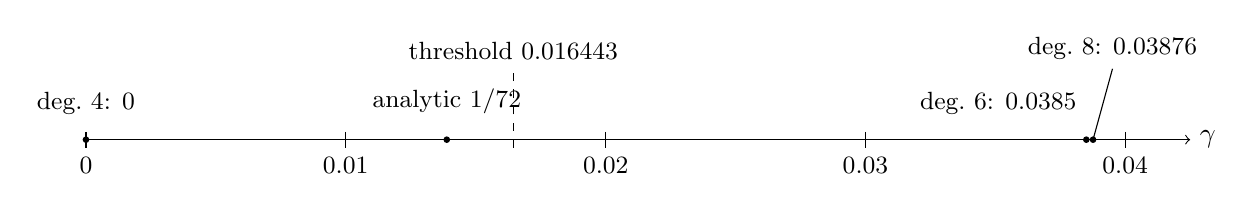
\begin{tikzpicture}[x=330cm,y=1mm]
  \draw[->] (0,0) -- (0.0425,0) node[right] {$\gamma$};
  \foreach \t in {0,0.01,0.02,0.03,0.04} \draw (\t,1) -- (\t,-1) node[below] {\small\t};
  \fill (0,0) circle (1.2pt); \node[above] at (0,2) {\small deg.\ 4: $0$};
  \fill (0.013889,0) circle (1.2pt); \node[above] at (0.013889,2) {\small analytic $1/72$};
  \draw[dashed] (0.016443,-1) -- (0.016443,9); \node[above] at (0.016443,9) {\small threshold $0.016443$};
  \fill (0.0385,0) circle (1.2pt); \node[above left] at (0.0385,2) {\small deg.\ 6: $0.0385$};
  \fill (0.0387628,0) circle (1.2pt); \draw (0.0387628,0) -- (0.0395,9); \node[above] at (0.0395,9) {\small deg.\ 8: $0.03876$};
\end{tikzpicture}
\end{center}
The number line above shows the lower bounds on $\min\E_{\Tz}$ on a horizontal axis from $0$ to $0.04$: the
degree-four value $0$, the analytic bound $1/72\approx0.0139$, the certified degree-six bound $0.0385$, and the exact
degree-eight value $0.03876$, which sits just to the right of $0.0385$. The dashed line at $0.016443$ is the energy a
triple needs for the bias conclusion of Section~\ref{sec:sets}; the analytic bound lies below it, both certified
bounds lie above it.

\subsection{From a vector to a basis}\label{sec:bridge}

A lower bound on the energy of one vector is not yet a statement about a measurement. An experiment does not use a
single vector but a whole basis (a measurement with six outcomes), and the quantities used to compare sets of bases
are statements about whole bases. Two standard figures of merit are the \emph{bias} of a family of bases, the largest
deviation $\bigl|\abs{\ip ef}^2-\frac16\bigr|$ over pairs of vectors from different bases, and the score in the
random-access-code game of \cite{ABMP}. In the game a pair $(a,b)$ of the four bases is drawn uniformly from the six
pairs and announced; then the sender receives $x_1,x_2\in\{1,\dots,6\}$ uniformly and sends one six-level system,
and the receiver, asked for $x_1$ or $x_2$, measures in basis $a$ or $b$. With the optimal encoding the success
probability for the pair is $P_{ab}=\frac12+\frac1{72}\sum_{i,j}\abs{\ip{e^a_i}{e^b_j}}$ \cite{ABMP} \stcited, and
the score is the average of $P_{ab}$ over the six pairs. Four mutually unbiased bases would score
$\frac12+\frac{\sqrt6}{12}=0.7041241$; the \emph{game loss} of a set is $0.7041241$ minus its score. The following
lemma and theorem convert the energy bound into bounds on both quantities.

% ===== Core of Section 6.3. Include VERBATIM (you may add connecting prose before/after, not change the mathematics). =====
\begin{lemma}[A quadratic cap on the square root]\label{lem:sqrt}
Let $a=1/\sqrt6$ and $\cstar=\dfrac{3\sqrt6}{(\sqrt6+1)^2}=\dfrac{21\sqrt6-36}{25}=0.617571\ldots$ Then for every $p\in[0,1]$
\[
  \sqrt p\;\le\;\frac1{\sqrt6}+\frac{\sqrt6}{2}\Bigl(p-\frac16\Bigr)-\cstar\Bigl(p-\frac16\Bigr)^{2},
\]
with equality exactly at $p=1/6$ and $p=1$. \stproved\ \event
\end{lemma}
\begin{proof}
Write $s=\sqrt p\in[0,1]$, so $p-\tfrac16=s^2-a^2=(s-a)(s+a)$. The tangent line of the square root at $1/6$
exceeds it by a perfect square:
\[
  a+\frac{s^2-a^2}{2a}-s=\frac{(s-a)^2}{2a}.
\]
Hence the claim is $(s-a)^2\bigl[\tfrac1{2a}-\cstar\,(s+a)^2\bigr]\ge0$. Since $0\le s\le1$ we have
$(s+a)^2\le(1+a)^2$, and $\cstar$ was chosen as
$\cstar=\dfrac1{2a(1+a)^2}=\dfrac{\sqrt6/2}{(1+1/\sqrt6)^2}=\dfrac{3\sqrt6}{(\sqrt6+1)^2}$,
so the bracket is nonnegative and vanishes only at $s=1$. The first factor vanishes only at $s=a$.
\end{proof}

\begin{theorem}[From a vector to a basis]\label{thm:bridge}
Let $B_1,B_2,B_3$ be orthonormal bases of $\C^6$ (not assumed mutually unbiased) with vectors $v_{r,k}$, and
suppose that every unit vector $\psi$ satisfies $\E(\psi)=\sum_{r=1}^{3}\sum_{k=1}^{6}\bigl(\abs{\ip{v_{r,k}}{\psi}}^2-\tfrac16\bigr)^2\ge\gamma$
for some $\gamma>0$. Let $F=\{f_1,\dots,f_6\}$ be any fourth orthonormal basis. Then:
\begin{enumerate}[label=(\alph*)]
\item (\emph{Bias.}) For every $j$ there are $r,k$ with $\bigl|\abs{\ip{v_{r,k}}{f_j}}^2-\tfrac16\bigr|\ge\sqrt{\gamma/18}$.
      In particular the bias of $\{B_1,B_2,B_3,F\}$ is at least $\sqrt{\gamma/18}$.
\item (\emph{Game.}) The four-basis game score of $\{B_1,B_2,B_3,F\}$ is at most
      $\tfrac12+\tfrac{\sqrt6}{12}-\tfrac{\cstar\gamma}{72}$: it falls short of the value $\tfrac12+\tfrac{\sqrt6}{12}$ of four
      mutually unbiased bases by at least $\cstar\gamma/72$.
\end{enumerate}
\stproved\ \event
\end{theorem}
\begin{proof}
(a) $\E(f_j)\ge\gamma$ is a sum of $18$ nonnegative terms, so one of them is at least $\gamma/18$.

(b) Fix two orthonormal bases $\{e_i\}$, $\{g_j\}$ and put $p_{ij}=\abs{\ip{e_i}{g_j}}^2$. There are $36$ numbers
$p_{ij}\in[0,1]$ and $\sum_{i,j}p_{ij}=6$, so $\sum_{i,j}(p_{ij}-\tfrac16)=0$. Summing Lemma~\ref{lem:sqrt} over the $36$ pairs,
\begin{equation}\label{eq:pairsum}
  \sum_{i,j}\abs{\ip{e_i}{g_j}}=\sum_{i,j}\sqrt{p_{ij}}\;\le\;\frac{36}{\sqrt6}-\cstar\sum_{i,j}\Bigl(p_{ij}-\frac16\Bigr)^2
  =6\sqrt6-\cstar\sum_{i,j}\Bigl(p_{ij}-\frac16\Bigr)^2 .
\end{equation}
For the three pairs $(B_r,F)$, $r=1,2,3$, the sums of squares on the right add up to
$\sum_{j=1}^{6}\E(f_j)\ge6\gamma$. For the three pairs inside the triple we drop the (nonnegative) square term and keep
$6\sqrt6$. The score is $\tfrac12+\tfrac1{72}\cdot\tfrac16\sum_{\text{6 pairs}}\sum_{i,j}\abs{\ip{e_i}{g_j}}$, hence
\[
  \text{score}\;\le\;\frac12+\frac1{72}\cdot\frac{6\cdot6\sqrt6-6\cstar\gamma}{6}=\frac12+\frac{\sqrt6}{12}-\frac{\cstar\gamma}{72}.\qedhere
\]
\end{proof}

\begin{remark}[What the proof uses]\label{rem:bridgeuses}
Only two inputs enter: the elementary Lemma~\ref{lem:sqrt}, and a lower bound $\gamma$ on the energy of a single
vector. Part (b) does not use that the triple is mutually unbiased, and it applies vector by vector, so it also bounds
the score of a partial fourth basis. Inequality~\eqref{eq:pairsum} with the square term dropped is the familiar statement
that a pair of bases maximizes $\sum\abs{\ip{e_i}{g_j}}$ exactly when it is mutually unbiased; the square term makes
that statement quantitative.
\end{remark}

\begin{corollary}[Numbers for the two product triples]\label{cor:numbers}
With the certified bounds of Proposition~\ref{prop:cert6}:
for $\Tz$ ($\gamma=0.0385$) every fourth basis has bias $>0.046248$ and game loss $>3.302\times10^{-4}$;
for $\To$ ($\gamma=0.0235$) every fourth basis has bias $>0.036132$ and game loss $>2.015\times10^{-4}$.
\stproved\ from \stcert\ inputs \event
\end{corollary}
% ===== end of verbatim core =====

The four numbers of Corollary~\ref{cor:numbers} are $\sqrt{\gamma/18}$ and $\cstar\gamma/72$ evaluated in Arb ball
arithmetic by \texttt{verify\_sets.py} ($0.046248$, $3.302291\times10^{-4}$, $0.036132$, $2.015684\times10^{-4}$, each a
rigorous lower end, then rounded down) \stcert\ \event. Independent numerical checks agree with the lemma and the
theorem \stnum\ \event. On $1.8$ million random probability vectors $(p_1,\dots,p_6)$ (Dirichlet distributions with
six concentration parameters from $0.05$ to $500$, $300{,}000$ vectors each), the summed form
$\sum_i\sqrt{p_i}\le\sqrt6-\cstar\sum_i(p_i-\frac16)^2$ of Lemma~\ref{lem:sqrt} always holds, with smallest slack
$1.6\times10^{-6}$; a Nelder--Mead search for a violation of the pointwise inequality from $2{,}000$ random starts in
$[0,1]$ finds smallest slack exactly $0$, attained at the equality points. For the game, the best fourth basis for
$\Tz$ found by numerical optimisation loses $1.506\times10^{-3}$, which is consistent with (and about $4.6$ times) the
proved lower bound $3.302\times10^{-4}$; for the bias, the best fourth basis for $\Tz$ found in $40$ random starts has
bias $0.0798$, consistent with the proved lower bound $0.046248$.

\subsection{Explicit four-basis sets and a design lesson}\label{sec:sets}

Upper bounds on the best possible bias or game loss come from explicit sets. We use two sets of four orthonormal
bases of $\C^6$ that were found earlier in the event by workstream A by numerical optimisation over all quadruples
of bases \stnum\ \event. The first set (file \texttt{bases\_d6\_delta.npy}) minimises the bias: it was the best of
$72$ starts (random starts, star-shaped starts, a mutually unbiased triple plus a random fourth basis, and
previously saved sets); in it all six pairs
of bases attain the maximal deviation and no pair is exactly unbiased. The second set (file
\texttt{bases\_d6\_P4.npy}) maximises the game score: it was the best of $700$ starts (random and seeded with a
mutually unbiased triple), and its score $0.7038884$ reproduces the value quoted in the review \cite{MWreview}
\stcited. In that set one basis is unbiased to the other three and the remaining three pairs are slightly biased,
so it contains no exactly mutually unbiased triple. (The same study also reproduced the ``four most distant bases''
of Raynal, L\"u and Englert \cite{RLE}, which optimise an average squared distance; that set is not used here.)

The sets are stored in double precision, so the stored matrices $\tilde B$ are unitary only up to rounding. The
checker \texttt{verify\_sets.py} therefore applies a \emph{unitarity correction}. For each stored matrix it computes
in ball arithmetic $\varepsilon=\norm{\tilde B^{\dagger}\tilde B-I}_F$ (all eight matrices have
$\varepsilon\le4.4\times10^{-15}$). The polar factor $U$ of $\tilde B$ is an exactly unitary matrix with
$\norm{U-\tilde B}_2\le\varepsilon$, and the statements are made about these exact bases $U$. For a pair of bases
$a,b$ the overlaps of the exact bases differ from the stored overlaps by at most
$t=(\varepsilon_a+\varepsilon_b)(1+\varepsilon_{\max})$, and the squared overlaps by at most
$t\bigl(2(1+\varepsilon_{\max})^2+t\bigr)$; these amounts are added to every upper bound on a deviation and
subtracted from every overlap modulus entering the game score. All other arithmetic is in Arb balls at 160 bits.
The result \stcert\ \event:
\begin{itemize}
\item the exact bases of \texttt{bases\_d6\_delta.npy} have bias $\le0.030223872$ (and game loss
      $\le6.180869\times10^{-4}$);
\item the exact bases of \texttt{bases\_d6\_P4.npy} have game loss $\le2.357825\times10^{-4}$ (and bias
      $\le0.040598665$).
\end{itemize}
These are upper bounds on the smallest possible bias and the smallest possible game loss over all quadruples of
bases. No positive lower bound for either is known: the 2026 proofs imply that both are positive but give no value.

\begin{corollary}[Design lesson]\label{cor:design}
\begin{enumerate}[label=(\alph*)]
\item Every set of four orthonormal bases of $\C^6$ that contains the canonical product triple $\Tz$ has bias
      $>0.046248>0.030224$ and game loss $>3.302\times10^{-4}>2.358\times10^{-4}$. Hence the explicit sets beat every
      completion of $\Tz$ on both measures, and no bias-optimal or game-optimal quadruple contains $\Tz$.
\item Every set of four bases containing $\To$ has bias $>0.036132>0.030224$, so no bias-optimal quadruple contains
      $\To$.
\end{enumerate}
\stproved\ from \stcert\ inputs \event
\end{corollary}
\begin{proof}
Combine Corollary~\ref{cor:numbers} with the certified upper bounds for the two explicit sets.
\end{proof}

In words: the best approximate quadruples are \emph{not} completions of the perfect local triple (the qubit triple
tensored with the qutrit triple). Building a four-basis experiment by keeping the three product bases exactly and
adding the best possible fourth basis is provably worse than the best known sets. For $\To$ and the game the
comparison is \emph{inconclusive}: the proved loss bound $2.015\times10^{-4}$ is smaller than the loss
$2.358\times10^{-4}$ of the explicit set, so our numbers do not exclude that a completion of $\To$ is at least as
good in the game \stconj.

The bias part of the lesson needs very little from a triple. By Theorem~\ref{thm:bridge}(a), any triple with
$\E\ge\gamma$ everywhere forces bias $\ge\sqrt{\gamma/18}$ on its completions, and $\sqrt{\gamma/18}>0.030223872$ as
soon as $\gamma\ge0.016443$ (since $18\times0.030223872^2=0.0164427\ldots$) \stproved. Both product triples clear
this threshold with room to spare, and the analytic bound $1/72$ does not.

The next natural family is the dimension-six Fourier pair $\{I,F_6\}$. Workstream A certified the $48$ vectors
unbiased to both $I$ and $F_6$, found $300$ orthogonal pairs among them and $16$ third bases completing the pair to a
mutually unbiased triple \stcert\ \event; that these $48$ are all such vectors rests on the published count of
$156$ cyclic $6$-roots \cite{BF91,Grassl} \stcited. The numerical energy minima of the $16$ triples are $0.0326759$
($12$ triples), $0.0238354$ ($2$ triples) and $0.0387628$ ($2$ triples) \stnum.

\begin{proposition}[Energy certificates for all triples containing the Fourier pair]\label{prop:fourier6}
For each of the $16$ triples $\{I,F_6,B\}$, every unit vector $\psi\in\C^6$ has
$\E(\psi)>0.0323999$ ($12$ triples), $\E(\psi)>0.0234999$ ($2$ triples), or $\E(\psi)>0.0384999$ ($2$ triples).
In particular $\E\ge0.0234999$ for every mutually unbiased triple that contains $\{I,F_6\}$.
\stcert\ \event
\end{proposition}

\noindent\emph{How it was obtained.} The same degree-six certificate as in Proposition~\ref{prop:cert6}, built and
checked by the general-triple scripts of Appendix~\ref{app:cert}. The third-basis vectors enter the checker as
complex balls of radius $10^{-30}$ that are re-certified inside the script (Krawczyk test and unimodularity test at
200 bits), so the bound holds for the true vectors, not for their floating-point approximations. All $16$
certificates pass; the smallest certified value is $0.0234999999946$, the largest residual absorbed is
$5.8\times10^{-12}$. Re-checking the $16$ stored Gram matrices takes $12$ seconds
(\texttt{d6\_fourier/verify\_fourier6\_certs.py}); finding them took about two minutes per triple.

\begin{corollary}[Design lesson for the Fourier pair]\label{cor:fourier6}
Any four orthonormal bases of $\C^6$ that contain a mutually unbiased triple $\{I,F_6,B\}$ have bias greater than
$0.036132$, which exceeds the bias $0.030224$ of the explicit quadruple. So the least-biased quadruples known are
not completions of any triple containing the Fourier pair either. \stproved\ from \stcert\ inputs, given the cited
classification of the $48$ vectors \event
\end{corollary}

\noindent For the game the comparison is conclusive only for the $14$ triples with $\gamma\ge0.0323999$: there the
loss is at least $\cstar\cdot0.0323999/72>2.779\times10^{-4}>2.358\times10^{-4}$. For the two triples with
$\gamma=0.0234999$ it is inconclusive, as for $\To$.


\subsection{Hide and seek: a detection test}\label{sec:hide}

The energy has a direct operational meaning. Consider a game between a \emph{hider} and a \emph{referee}. The hider
prepares, again and again, the same pure state $\psi$ of a qubit and a qutrit, and tries to make it look like white
noise to the three local measurements of $\Tz$ (qubit in the $Z$, $X$ or $Y$ eigenbasis, qutrit in the
corresponding basis $I_3$, $F_3$ or $DF_3$). The referee takes $N$ shots in each of the three settings and applies
Pearson's chi-square test for uniformity to the $3\times6$ table of counts, with $3\times5=15$ degrees of freedom and
false-alarm rate $0.1\%$ (the probability of declaring non-uniformity for truly uniform data). A complete set of
mutually unbiased bases extending $\Tz$ would contain a state with $\E=0$, which the referee could never catch.

\paragraph{Shot counts.} For outcome probabilities $p_{r,k}$, the Pearson statistic is asymptotically a noncentral
chi-square variable with $15$ degrees of freedom and noncentrality
$\lambda=\sum_{r}N\sum_k(p_{r,k}-\frac16)^2/(1/6)=6N\E(\psi)$ \stproved. So $\E$ is the detectability per shot, the
minimum-energy state is the best hider, and the certified bound $\E\ge0.0385$ of Proposition~\ref{prop:cert6} gives
a floor $\lambda\ge6N\times0.0385$ for \emph{every} pure state. From this floor, using the noncentral chi-square
distribution (\texttt{scipy.stats.ncx2}) \stcomp\ \event:
\begin{itemize}
\item $239$ shots per setting give detection probability at least $99\%$ at false-alarm rate $0.1\%$;
\item at a one-sided five-sigma false-alarm rate ($2.87\times10^{-7}$), $198$ shots per setting give $50\%$
      detection and $369$ give $99\%$ (the continuous solution is $N=368.07$).
\end{itemize}
\textbf{These shot counts are not a finite-sample theorem.} They use the large-$N$ chi-square approximation to the
distribution of the Pearson statistic, checked by Monte Carlo simulation; the only rigorous input is the bound on
$\E$. In the simulation the referee's false-alarm rate on exactly uniform data was $0.00094$, $0.00085$, $0.00100$,
$0.00093$ at $N=10,30,100,1000$ ($200{,}000$ trials each; target $0.001$), and simulated detection rates of the best
hider at $28$ values of $N$ from $10$ to $5{,}000$ ($20{,}000$ trials each) follow the noncentral chi-square
prediction (for example $0.476$ against $0.487$ at $N=100$ and $0.963$ against $0.960$ at $N=199$) \stcomp\ \event.

\paragraph{Circuits and noise.} The six-level system is one physical qubit plus a qutrit stored in two qubits (the
fourth level $|11\rangle$ unused; outcomes there are discarded). Every setting is a product measurement, so measuring
needs no entangling gate between the qubit and the qutrit: after transpilation to $\{\mathrm{cx},u\}$ the three
measurement circuits use $0$, $3$ and $3$ CNOT gates, all inside the qutrit's two qubits, and preparation plus
measurement uses $4$, $7$ and $7$ \stcomp\ \event. We simulated these circuits (Qiskit Aer, density-matrix method,
depolarising error $r$ on each CNOT and $r/10$ on each one-qubit gate, shot noise by multinomial sampling, fixed
seeds), with the minimum-energy state $\psi_\ast$ as hider. Noiseless circuits reproduce the exact probabilities to
$5.3\times10^{-16}$. The total number of shots (over the three settings) for $50\%$ detection at five-sigma false
alarm, computed from the energy of the simulated noisy state, is $589$ without noise ($3\times196.2$), $594$ at
two-qubit error $0.1\%$, $646$ at $1\%$, and $1{,}500$ at $10\%$, where the noisy state's energy has dropped to
$0.0152$ \stcomp\ \event.

\paragraph{The control in dimension four.} In $\C^4$ with two qubits and settings $ZZ$, $XX$, $YY$, the state
$(1,1,i,-i)/2$ is exactly uniform in all three settings ($\E=0$ up to $10^{-31}$), because these three bases are part
of a complete set of five mutually unbiased bases. The referee (now with $9$ degrees of freedom) never catches it:
its detection rate stays at the false-alarm rate $0.001$ up to $5{,}000$ shots per setting, at every noise level
tried ($20{,}000$ trials per point) \stcomp\ \event. This is what a complete set looks like to the test; dimension
six is different.

\begin{figure}[ht]\centering
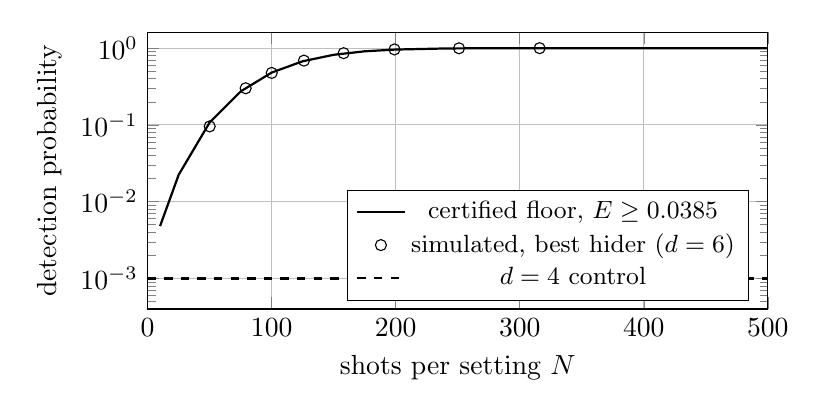
\begin{tikzpicture}
\begin{axis}[width=0.78\textwidth,height=0.42\textwidth,xmin=0,xmax=500,ymode=log,ymin=4e-4,ymax=1.6,
  xlabel={shots per setting $N$},ylabel={detection probability},legend pos=south east,
  legend style={font=\small},grid=major]
\addplot[thick,black] coordinates {(10,0.0048) (25,0.0224) (50,0.1078) (75,0.2733) (100,0.4812) (125,0.6751)
  (150,0.8197) (175,0.9102) (200,0.9594) (239,0.9901) (250,0.9935) (300,0.9992) (350,0.9999) (400,1.0) (500,1.0)};
\addlegendentry{certified floor, $\E\ge0.0385$}
\addplot[only marks,mark=o] coordinates {(50,0.0957) (79,0.30025) (100,0.47565) (126,0.6884) (158,0.8604)
  (199,0.9628) (251,0.9957) (316,0.9998)};
\addlegendentry{simulated, best hider ($d=6$)}
\addplot[thick,dashed] coordinates {(0,0.001) (500,0.001)};
\addlegendentry{$d=4$ control}
\end{axis}
\end{tikzpicture}
\caption{Detection probability of the chi-square referee at false-alarm rate $0.1\%$ against the number of shots per
setting.}\label{fig:hide}
\end{figure}

Figure~\ref{fig:hide} shows the detection probability (vertical axis, logarithmic, from $4\times10^{-4}$ to $1$)
against the number $N$ of shots per setting (horizontal axis, $0$ to $500$), at false-alarm rate $0.1\%$. The solid
curve is the guaranteed floor for every pure state against $\Tz$, computed from the noncentral chi-square distribution
with $15$ degrees of freedom and noncentrality $6N\times0.0385$: it rises from $0.005$ at $N=10$ through $0.11$ at
$N=50$, $0.48$ at $N=100$ and $0.96$ at $N=200$, reaches $0.99$ at $N=239$, and is essentially $1$ beyond $N=350$. The
circles are Monte Carlo detection rates for the best hider $\psi_\ast$ (true energy $0.03876$, slightly above the
certified floor); they lie on or just above the curve. The dashed horizontal line at $0.001$ is the dimension-four
control, whose detection rate never rises above the false-alarm rate.

\paragraph{Limits.} The certified floor applies to pure states only. A mixed state can hide: the maximally mixed
state is exactly uniform in every basis and hides perfectly, and the noise scan above shows how much gate noise the
best pure hider needs before its energy falls well below the floor. The simulated noise is unbiased depolarising
noise; real devices have biased readout, which itself produces non-uniform counts, so an experiment needs a
calibration run on white noise before the test means anything. Finally, the simulation repeats linear algebra and
proves nothing by itself; its role is to translate the certified bound into shots and gate-error requirements.

\subsection{The game, for comparison}\label{sec:game}

The game of Section~\ref{sec:bridge} could also be used to see the missing basis, but it is far less sensitive. The
relevant gap is the game loss $\Delta=2.3578\times10^{-4}$ of the explicit set \texttt{bases\_d6\_P4.npy} (rigorously
$\Delta\le2.357825\times10^{-4}$, Section~\ref{sec:sets}), recomputed from the stored bases and from the earlier
simulation data of workstream A. Since no four bases can score more than the ideal value $\mu=\frac12+\frac{\sqrt6}{12}$
and the explicit set already scores $\mu-\Delta$, any experiment that tries to show a six-level device falls short of
$\mu$ must resolve a shortfall of at most $\Delta$. Two requirements follow \stcomp\ \event:
\begin{itemize}
\item \emph{Rounds.} With $n$ independent rounds the estimated success frequency has standard deviation
      $\sqrt{\mu(1-\mu)/n}$. Requiring the shortfall $\Delta$ to equal five standard deviations gives
      $n=25\,\mu(1-\mu)/\Delta^2=9.37\times10^{7}$ rounds ($9.3686\times10^{7}$).
\item \emph{Gate error.} In the simulated game (six-level system in three qubits, Qiskit Aer, same noise model as
      above, $200$ sampled settings), the noise lowers the score by about $20.3\,r$ when preparation and measurement are
      compiled separately (about $33$ CNOT gates per circuit) and by about $11.6\,r$ when they are fused ($19$ CNOT
      gates), with slopes measured at $r=10^{-6}$. The noise loss equals $\Delta$ at
      $r=1.16\times10^{-5}$ (separate) and $r=2.03\times10^{-5}$ (fused); above these two-qubit error rates noise alone
      costs more than the gap.
\end{itemize}
The earlier team report quoted $3.4\times10^{7}$ rounds and a noise level $4.4\times10^{-4}$ for the same gap. Both
differences are differences of criterion, not of data: $3.4\times10^{7}$ is the same formula at three standard
deviations instead of five ($9\mu(1-\mu)/\Delta^2$), and $4.4\times10^{-4}$ is the strength $\epsilon$ of a single
depolarising channel on the transmitted system at which the score $(1-\epsilon)P+\epsilon/6$ loses $\Delta$, that is
$\epsilon=\Delta/(\mu-\frac16)$, rather than an error rate per two-qubit gate. Here we use only the five-sigma round
count and the per-gate error rate defined above.

\paragraph{Conclusion.} The detection test needs about $6\times10^{2}$ shots in total, the game about $10^{8}$
rounds: five orders of magnitude more ($9.37\times10^{7}/589\approx1.6\times10^{5}$). The test also tolerates
two-qubit error rates of $1\%$ to $10\%$ at the cost of at most $2.6$ times more shots, where the game needs
about $10^{-5}$. The two numbers answer different
questions, however. The detection test certifies that one fixed triple, the canonical product triple, has no hidden
unbiased pure state; it says nothing about other triples. The game shortfall concerns every set of four bases, but
our numbers for it only bound the shortfall from above ($\Delta\le2.357825\times10^{-4}$); the 2026 proofs say the
smallest shortfall over all quadruples is positive without giving a value, so no round count for the game is a
guarantee.

% ======================= s7_ten =======================
\section{Dimension ten by the same method}\label{sec:ten}

\noindent\emph{Status of this section.} All dimension-ten computations here are workstream~A \event. The
headline (Theorem~\ref{thm:ten}) is a computer-assisted theorem that is conditional on a cited count of
complex solutions, hypothesis~(H) below, which we did not verify; it carries the tag \stcond. The certified
enumeration steps are \stcert, the orbit counts are \stcomp, the random-start searches and the energy minima
are \stnum, and literature is \stcited\ \prior. Method details are in Appendix~\ref{app:ten}.

\subsection{Why ten, and what is known}

Dimension $10=2\times5$ is the next dimension after $6=2\times3$ of the form $2\times(\text{odd prime})$, so it
is the natural next test of whether the dimension-six phenomenon persists. As in dimension six it has a
natural local triple: three mutually unbiased bases of a qubit ($\C^2$) tensored with three of a ququint
($\C^5$). Complete sets of $p+1$ MU bases exist in every prime dimension $p$, and $d+1$ is an upper bound in
every dimension $d$ \cite{WF} \stcited\ \prior. Tensoring three MU bases of $\C^2$ with three of $\C^5$ gives
three MU bases of $\C^{10}$, so $3\le N(10)\le 11$, where $N(d)$ is the largest number of MU bases in $\C^d$
\cite{WF,MWreview} \stcited\ \prior. Whether a fourth MU basis exists in $\C^{10}$ is open \cite{MWreview} \stconj\ \prior.
Nothing like the three 2026 computer proofs for dimension six (\cite{OAI,Jaswal1,CWT}) exists for dimension
ten. We therefore treat one well-defined slice of the problem, the triples that contain the pair formed by
the standard basis $I$ and the Fourier basis $F_{10}$ (columns of $F/\sqrt{10}$,
$F_{jk}=\omega^{jk}$, $\omega=e^{2\pi i/10}$), and carry the dimension-six Fourier computation
(\cite{Grassl}; recomputed in the earlier team report) over to it.

\subsection{The reduction to cyclic 10-roots}

\begin{definition}
A \emph{cyclic $n$-root} is a point $z\in\C^n$ with
\[
  \sum_{j=0}^{n-1}\ \prod_{i=0}^{k-1} z_{j+i}=0\quad(k=1,\dots,n-1),\qquad \prod_{j=0}^{n-1}z_j=1,
\]
indices taken mod $n$. It is \emph{unimodular} if $\abs{z_j}=1$ for all $j$.
\end{definition}

Let $v\in\C^{10}$ be unbiased to $I$ and $F_{10}$. Unbiased to $I$ means $\abs{v_j}^2=1/10$ for all $j$,
so after multiplying by a global phase and by $\sqrt{10}$ we may write $v=x/\sqrt{10}$ with $x_0=1$ and
$\abs{x_j}=1$. Unbiased to $F_{10}$ means $\abs{X_k}^2=10$ for all $k$, where $X_k=\sum_j\omega^{-jk}x_j$.
Now $\abs{X_k}^2=\sum_{s}c_s\,\omega^{-sk}$ with the periodic autocorrelation
$c_s=\sum_j x_{j+s}\overline{x_j}$, and $c_0=10$. By Fourier inversion, $\abs{X_k}^2=10$ for all $k$ holds if
and only if $c_s=0$ for $s=1,\dots,9$. Since $\overline{x_j}=1/x_j$ on the torus, these are the equations
$g_s(x)=\sum_j x_{j+s}/x_j=0$, $s=1,\dots,9$. Put $z_j=x_{j+1}/x_j$. Then
$\prod_{i<s}z_{j+i}=x_{j+s}/x_j$, so $g_s(x)=0$ is the $s$-th cyclic equation, and $\prod_j z_j=1$
automatically; conversely $x_0=1$, $x_{j+1}=x_jz_j$ inverts the map, and $\abs{x_j}=1$ for all $j$ if and only
if $\abs{z_j}=1$ for all $j$. Hence unit vectors unbiased to $I$ and $F_{10}$, up to a global phase, are in
bijection with unimodular cyclic 10-roots (a standard observation; see \cite{FR15}) \stcited\ \prior.

\subsection{The hypothesis and what holds without it}

\begin{center}
\fbox{\parbox{0.9\linewidth}{\textbf{Hypothesis (H).} The cyclic 10-roots system has at most $34{,}940$
solutions in $\C^{10}$ (in particular, finitely many).}}
\end{center}

\noindent The count $34{,}940$ is a Gr\"obner-basis computation attributed to Faug\`ere; we know it only
through the table in \cite{FR15} \stcited\ \prior. \textbf{We did not verify (H).} It rests on a reported
computer-algebra computation, not on a proof we could read. Workstream~A exhibits $34{,}940$ distinct,
simple (nonsingular) roots, each in its own certified box (Appendix~\ref{app:ten}) \stcert\ \event. So under
(H) these are all the roots, whether the published number counts multiplicity or not. Without (H), Bernstein's
theorem bounds the number of isolated roots in $(\C^*)^{10}$, with multiplicity, by the mixed volume of the
Newton polytopes. The mixed volume of cyclic~10 is $35{,}940$; this value was computed with PHCpack by an
auxiliary session of workstream~A and was not recomputed or found in a source we read \streported. Given that
value, at most $1{,}000$ further isolated roots can exist \stcond\ \event. Bernstein's bound does not exclude
positive-dimensional solution sets; (H) does.

\subsection{The funnel}

Table~\ref{tab:ten} lists the stages of the computation, with the dimension-six case as calibration.

\begin{table}[ht]
\centering
\small
\begin{tabular}{@{}lrr@{}}
\toprule
stage & $d=10$ & $d=6$ (calibration)\\
\midrule
complex cyclic $d$-roots (count used) & $34{,}940$, under (H) \cite{FR15} & $156$ \cite{BF91}\\
\quad certified distinct roots located & $34{,}940$ & $156$\\
unimodular roots = vectors unbiased to $I$, $F_d$ & $3{,}040$ (10 orbits) & $48$\\
possibly orthogonal pairs among them & $57{,}680$ & $300$\\
candidate third bases ($d$-cliques) & $1{,}136$ (19 orbits) & $16$\\
pairs of candidate bases that are MU & $0$ & $0$\\
vectors unbiased to some triple $\{I,F_d,B\}$ & $0$ & $0$\\
\bottomrule
\end{tabular}
\caption{The funnel. Dimension ten: workstream~A, certified steps conditional on (H) \stcond\ \event.
Dimension six: the same pipeline (\texttt{d6f/fourier6.py}; earlier team report), conditional on the classical
count $156$ \cite{BF91}, agreeing with \cite{Grassl} \stcert\ \event. Orbits are under the group of order
$1600$ described in Appendix~\ref{app:ten}.}
\label{tab:ten}
\end{table}

\begin{center}
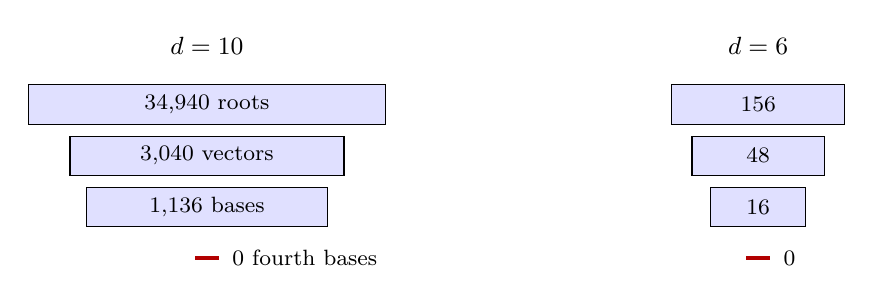
\begin{tikzpicture}[x=1cm,y=1cm,
  st/.style={draw,fill=blue!12,minimum height=0.5cm,inner sep=1pt,font=\footnotesize}]
  \node[font=\small\bfseries] at (0,0.75) {$d=10$};
  \node[st,minimum width=4.54cm] at (0,0) {34{,}940 roots};
  \node[st,minimum width=3.48cm] at (0,-0.65) {3{,}040 vectors};
  \node[st,minimum width=3.06cm] at (0,-1.30) {1{,}136 bases};
  \draw[very thick,red!70!black] (-0.15,-1.95) -- (0.15,-1.95);
  \node[font=\footnotesize,right] at (0.2,-1.95) {0 fourth bases};
  \node[font=\small\bfseries] at (7,0.75) {$d=6$};
  \node[st,minimum width=2.19cm] at (7,0) {156};
  \node[st,minimum width=1.68cm] at (7,-0.65) {48};
  \node[st,minimum width=1.20cm] at (7,-1.30) {16};
  \draw[very thick,red!70!black] (6.85,-1.95) -- (7.15,-1.95);
  \node[font=\footnotesize,right] at (7.2,-1.95) {0};
\end{tikzpicture}
\end{center}

\noindent The inline figure draws each stage as a bar whose width is proportional to $\log_{10}$ of the count
(1~cm per decade): for $d=10$ the bars have widths $4.54$, $3.48$ and $3.06$~cm ($34{,}940$ roots, $3{,}040$
vectors, $1{,}136$ bases), for $d=6$ they have widths $2.19$, $1.68$ and $1.20$~cm ($156$, $48$, $16$). Both
funnels end in a short red mark labeled $0$: no candidate third basis admits a fourth basis, or even a single
further vector. The shapes are similar; dimension ten is about $2.35$ decades wider at the top and $1.85$
decades wider at the bases stage.

\subsection{What is certified, and how}

\emph{Roots.} The $34{,}940$ roots were found by damped Newton iteration from random starts and closure under
symmetries (a heuristic step that need not be rigorous), then each was enclosed by a Krawczyk test in Arb ball
arithmetic, which proves a unique root in each box; the boxes are pairwise disjoint \stcert\ \event. A
fixed-point test for the involution $x\mapsto 1/\overline{x}$ certifies exactly $3{,}040$ of them unimodular
and the other $31{,}900$ not unimodular \stcert\ \event. A second implementation reproduced the $34{,}940$
certified roots and the $3{,}040/31{,}900$ split \stcert\ \event. The $3{,}040$ unimodular roots were known
numerically before, with the same orbit sizes, without a proof of completeness \cite{FR15} \stcited\ \prior.

\emph{Availability.} The list of all $34{,}940$ certified roots and their certificates was produced in a separate
working session of workstream~A during the event and is not included in the submission repository. The
certification of the $31{,}900$ roots as not unimodular is therefore not reproducible from the repository and
should be read as \streported. The repository contains the $3{,}040$ unimodular roots; it re-certifies them and
recomputes everything downstream from scratch (\texttt{d10/check\_d10.py}).

\emph{Re-check by our own code.} A separate program (\texttt{d10/check\_d10.py}), which reads only the list of
$3{,}040$ points and, for comparison, the stored list of bases, re-certified all $3{,}040$ of $3{,}040$ points
as unimodular roots with its own Krawczyk and fixed-point tests (200-bit Arb, box half-width $10^{-30}$)
\stcert\ \event. It found exactly $57{,}680$ pairs whose inner-product enclosure contains $0$; every other pair
has $\abs{\ip{u}{v}}\ge 0.0089515$ in the scaling $\abs{u_j}=\abs{v_j}=1$, far above the double-precision
error bound $10^{-13}$ \stcert\ \event. Its own clique enumeration finds no clique larger than $10$ and
exactly $1{,}136$ ten-cliques, identical to the stored list \stcomp\ \event.

\emph{Exactness.} An enclosure that contains $0$ does not prove orthogonality, so the $1{,}136$ are
\emph{candidates}. That all of them are bases is \stnum\ (enclosures of radius about $10^{-40}$ containing $0$).
For $96$ of them (orbits of product and cyclotomic type) orthogonality was proved exactly in $\mathbb{Q}(\zeta_{20})$
\stcomp\ \event. Theorem~\ref{thm:ten} does not need exactness: every true basis is among the candidates.

\begin{theorem}[conditional]\label{thm:ten}
Assume (H). Every orthonormal basis $B$ of $\C^{10}$ that is unbiased to both $I$ and $F_{10}$ is, up to the
order and phases of its vectors, one of $1{,}136$ explicit candidate sets. For each of these $1{,}136$ sets $B$
and each unit vector $v$ unbiased to $I$ and $F_{10}$, some $b\in B$ satisfies
\[
  \Bigl|\,\abs{\ip{b}{v}}^2-\tfrac1{10}\Bigr|\ \ge\ 0.04178 .
\]
Equivalently, with all vectors scaled to unimodular entries ($\norm{u}^2=\norm{v}^2=10$),
\[
  \min_{B,\,v}\ \max_{u\in B}\ \bigl|\abs{\ip{u}{v}}^2-10\bigr|\ \ge\ 4.17807 ,
\]
the minimum running over the $1{,}136$ candidate sets and the $3{,}040$ vectors. Consequently no triple
$\{I,F_{10},B\}$ of MU bases is extended by even one further vector, and no set of four mutually unbiased bases
of $\C^{10}$ contains the pair $\{I,F_{10}\}$. \stcond\ \event\ (computer-assisted; conditional on (H))
\end{theorem}

\begin{proof}[Proof structure]
By the reduction, a unit vector unbiased to $I$ and $F_{10}$ is, up to phase, $x/\sqrt{10}$ for a unimodular
cyclic 10-root. Under (H) the $34{,}940$ certified boxes contain all roots, so such $x$ lies in one of the
$3{,}040$ certified boxes, of radius at most $10^{-30}$. The vectors of a basis $B$ unbiased to $I$ and $F_{10}$
are such vectors and are pairwise orthogonal, so each pair has an enclosure containing $0$; hence $B$ is a
$10$-clique of the possibly-orthogonal graph, and the clique enumeration lists all of them. For the margin, a
finite check runs over all $1{,}136\times3{,}040$ pairs $(B,v)$ and, for each, over the ten $u\in B$; the
smallest value of $\max_{u}\bigl|\abs{\ip{u}{v}}^2-10\bigr|$ is $4.1780746$, the error being bounded as in
Appendix~\ref{app:ten}. The minimum is attained at a vector $v\notin B$; for $v\in B$ the defect is $90$
(take $u=v$). If $\{I,F_{10},B,B'\}$ were MU, every vector of $B'$ would be unbiased to $I$, $F_{10}$ and $B$,
contradicting the margin.
\end{proof}

The theorem says more than ``no fourth basis'': every triple containing $\{I,F_{10}\}$ is strongly
unextendible, with a quantitative gap. The same margin, $4.17807$, is also the minimum over pairs of distinct
candidate bases of the largest defect between them \stcomp\ \event. The $1{,}136$ candidates fall into $19$
orbits under the symmetry group; $16$ candidates (5 orbits) are product bases, among them eigenbases of the
Weyl operators $XZ^{\pm1}$ and $XZ^{\pm3}$, and the other $1{,}120$ are neither product bases nor Weyl
eigenbases \stnum\ \event. In dimension seven the same pipeline is a positive control: it finds $924$ roots,
$532$ vectors, $146$ bases, and recovers the complete set of $8$ MU bases \stcomp\ \event.

\subsection{Independent numerical evidence for completeness}

Since (H) is the weak point, we ran a search that does not use cyclic roots at all: Levenberg--Marquardt
least squares on the nine phases of $x$, minimizing $\sum_k(\abs{X_k}^2-10)^2$, from $1.2$ million uniformly
random starting phases (\texttt{d10/search\_match.py}, 60 batches of 20{,}000). Of these, $1{,}199{,}148$
converged (residual below $10^{-18}$), and every end point lies within $10^{-6}$ of the certified list (worst
distance $1.1\times10^{-9}$): none is off the list. Every one of the $3{,}040$ vectors was hit, at least $132$
times (median $326$, maximum $2{,}647$) \stnum\ \event. This is evidence for (H), not a proof: a solution with a
tiny basin of attraction, or a positive-dimensional family, could be missed.

\subsection{Limits}

\begin{itemize}
\item Theorem~\ref{thm:ten} concerns only triples containing the pair $\{I,F_{10}\}$. Other pairs of MU bases
in $\C^{10}$ have been explored numerically only \stnum\ \event. A ball certificate for further pairs whose
unbiased vectors saturate the count is unfinished: so far $1{,}552$ unimodular vectors are certified and $8$ are
undecided, against $1{,}560$ found numerically. We draw no conclusion from it \stconj\ \event.
\item The margin concerns vectors unbiased to $I$ and $F_{10}$. For an arbitrary state we have only numbers.
Write $\E(\psi)=\sum(p-\tfrac1{10})^2$ over the $30$ outcome probabilities of the triple. For the local
(product) triple, orbit 14, random-start L-BFGS (150 starts per orbit, \texttt{d10/energy10.py}) gives
$\min\E\approx0.0202$, so some outcome is off by at least about $0.026$. In the detection test of
Section~\ref{sec:hide} this corresponds to about $325$ shots per setting for $99\%$ detection at $0.1\%$ false
alarm \stnum\ \event. This is a numerical upper estimate of the minimum, so the true shot count could be
larger. Several non-product classes have much smaller numerical minima (smallest $0.0022$, orbit 8, about
$3{,}000$ shots), and some classes were reached by only $2$ to $5\%$ of starts (orbits 1, 7, 12), so these
minima are less reliable \stnum\ \event. No certified energy bound in dimension ten exists yet \stconj\ \event.
\item \cite{GMMP17} studied small unextendible sets of observables built from Weyl--Heisenberg operators,
including even composite dimensions. Our team ledger records that its statement covering the Weyl--Heisenberg
triple in dimension ten was not interval-certified and is contained, as a special case, in
Theorem~\ref{thm:ten} (orbit 14) \stcited\ \prior. We have not compared the precise wording.
\item The theorem is conditional on (H), and the mixed-volume bound above rests on a reported, not
recomputed, value.
\end{itemize}

The same three steps carry over from six to ten: certified enumeration, a certified margin, and a number an
experimentalist can use. What is missing in dimension ten is a proof that the list of roots is complete.

% ======================= 08_back =======================
\section{How each main claim is supported}\label{sec:support}

\emph{Status of this section.} One row per main claim, with the status tag, what exactly supports it, and
where to find it. ``Path'' refers to the submission repository. Nothing in this table is new; it is an index.

{\small
\begin{longtable}{@{}p{0.04\textwidth}p{0.36\textwidth}p{0.16\textwidth}p{0.36\textwidth}@{}}
\caption{Claims, status and support. A = certificate audit, energy certificate, bridge, detection test,
dimension ten; B = structure theory and Lean; C = explanatory audit and full rerun.}\label{tab:support}\\
\toprule
\# & Claim & Status & Support (what was done, range, path)\\
\midrule
\endfirsthead
\toprule
\# & Claim & Status & Support (what was done, range, path)\\
\midrule
\endhead
\bottomrule
\endfoot
1 & Three 2026 preprints claim that at most three MUBs exist in $\C^6$; none is formal end to end
  (Section~\ref{sec:trust}) & cited; read & Preprints and repositories read by A, B, C. Reading is not
  verification. The formal part of \cite{OAI} proves an upper bound of five only.\\
2 & The record checker of \cite{OAI} detects 17 of 26 deliberate corruptions (Section~\ref{sec:checks}) &
  computed & A. 26 mutations of the saved records, one run each; list in
  \texttt{near\_misses/repo/results/openai\_check/}.\\
3 & Full native rerun of \cite{OAI}: 100 invocations, 8 principal files byte-identical; $27{,}188$ root records
  re-certified at 128-bit precision (Section~\ref{sec:checks}) & reported, not re-run & C, audit commit
  \texttt{4360b1a5\ldots} of the team Lean repository. A did not rerun it.\\
4 & Sharp phase-ball radius $s^\ast=\sqrt6\arccos(1/\sqrt6)/(4\pi)$ (Section~\ref{sec:checks}) & proved &
  C, proof in the supplementary audit; A read the proof and checked the value numerically to 5 digits. Not used
  downstream.\\
5 & Cube-rank criterion: $\operatorname{rank}\hcube{H}\le2$ iff Fourier family, transpose, or Tao class
  (Section~\ref{sec:structure}) & proved, with one cited ingredient; computed & B. Reduction to a cited subblock
  classification; exact enumeration of $1{,}395$ systems, counts reproduced by A (\texttt{checks/check2.py}).\\
6 & Cubic norm cap $\norm{\hcube{H}}^2\le18$ for every order-six Hadamard matrix outside the Tao class, with
  the trace bound $\operatorname{tr}((M^\ast M)^2)\le648$, equality iff cube rank two; sharp six-phase bound
  (Section~\ref{sec:structure}) & proved, with one cited ingredient & B. Proofs in Section~\ref{sec:structure}; the
  Fourier condition used is cited from \cite{CWT}. Whether norm equality forces cube rank two is open. Six-phase
  bound spot-checked by A on 600 feasible points.\\
7 & Degree-four sum-of-squares relaxation has optimum $0$; pseudomoment matrix of rank 63
  (Section~\ref{sec:structure}) & computed (exact, B); reproduced numerically (A) & \texttt{checks/sos.py 4}.\\
8 & Universal vanishing of the residual products (Section~\ref{sec:structure}) & open & Not proved. No
  statement about the maximum number of MUBs follows from Section~\ref{sec:structure}.\\
9 & $\E>1/72$ on the canonical product triple (Appendix~\ref{app:gap}) & Lean-checked, as reported & B.
  Lean build run by B; A read the proof, did not run the build. Declarations in Table~\ref{tab:lean}.\\
10 & $\E\ge0.0385$ on $\Tz$ and $\E\ge0.0235$ on $\To$ for every unit vector (Section~\ref{sec:gap}) &
  interval-certified & A. Degree-six certificate checked in ball arithmetic: \texttt{cert/verify.py}
  (2 s per triple). The checker prints $0.038499999998$ and $0.023499999997$.\\
11 & The exact minimum on $\Tz$ is $(4-\sqrt6)/40$ (Section~\ref{sec:gap}) & cited & Prior work
  \cite{Erlwein}. Not ours. Our certificate reaches $99.3\%$ of it at lower degree.\\
12 & Lemma~\ref{lem:sqrt} and Theorem~\ref{thm:bridge}: a one-vector energy bound gives a bias bound and a game
  bound for every fourth basis (Section~\ref{sec:bridge}) & proved here & A. Complete proof in the text.
  Lemma also tested on $1.8$ million random points (\texttt{checks/check\_sqrt\_lemma.py}). LEAN-STATUS-PLACEHOLDER\\
13 & Any fourth basis added to $\Tz$: bias $>0.046248$, game loss $>3.302\times10^{-4}$; added to $\To$: bias
  $>0.036132$, game loss $>2.015\times10^{-4}$ (Corollary~\ref{cor:numbers}) & proved, from certified inputs &
  Rows 10 and 12.\\
14 & Explicit quadruples: bias $\le0.030223872$; game loss $\le2.357825\times10^{-4}$
  (Section~\ref{sec:sets}) & interval-certified & A. \texttt{cert/verify\_sets.py} on the two stored sets.\\
15 & Design lesson: the best approximate quadruples do not contain the canonical product triple
  (Section~\ref{sec:sets}) & proved, from certified inputs & Rows 13 and 14. For $\To$: proved for bias,
  inconclusive for the game.\\
16 & Detection test: 239 shots per setting for $99\%$ detection at $0.1\%$ false alarm
  (Section~\ref{sec:hide}) & computed & A. Certified energy bound plus the large-sample chi-square law, checked by
  Monte Carlo simulation. Not a finite-sample theorem. \texttt{hide\_seek/}.\\
17 & Resolving the game loss of the explicit quadruple needs $9.37\times10^{7}$ rounds
  (Section~\ref{sec:game}) & computed & A. \texttt{hide\_seek/RESULTS.md}.\\
18 & $\{5,4,4,1\}_6$ and $\{5,5,3,1\}_6$ of the 2008 table: the minimizer reaches strict local minima with
  nonzero misfit (Section~\ref{sec:const}) & interval-certified & A. \texttt{near\_misses/}; certificate rerun
  passes; independent 60-digit evaluation agrees.\\
19 & $\{5,3,3,3\}_6$ is found once in $20{,}000$ random starts (Section~\ref{sec:const}) & computed & A. One
  seed, $20{,}000$ starts; run record in \texttt{near\_misses/}.\\
20 & Dimension six, Fourier pair: every one of the $16$ triples containing $\{I,F_6\}$ has $\E\ge0.0234999$, so
  every fourth basis added to one of them has bias $>0.036132$ (Proposition~\ref{prop:fourier6},
  Corollary~\ref{cor:fourier6}) & interval-certified, given a cited classification & A. 16 certificates,
  third-basis vectors as certified balls: \texttt{d6\_fourier/verify\_fourier6\_certs.py} (12 s). Completeness of
  the $48$ vectors is cited \cite{BF91,Grassl}.\\
21 & Dimension ten: no four MUBs contain $\{I,F_{10}\}$ (Theorem~\ref{thm:ten}) & conditional & A. Conditional on
  hypothesis (H), the cited root count. $3{,}040$ vectors, $1{,}136$ candidate bases, margin $0.04178$ in probability, re-evaluated in ball arithmetic:
  \texttt{d10/}.\\
22 & Dimension ten: minimum energy $0.0202$ for the product-basis orbit (Section~\ref{sec:ten}) & numerical
  only & A. Upper estimate from local minimization; no certificate.\\
\end{longtable}
}

\section{Limitations and next steps}\label{sec:limits}

\emph{Status of this section.} Plain statements of what this report does not establish.

\begin{enumerate}[leftmargin=1.6em]
\item \textbf{We did not verify any of the three 2026 proofs.} Our checks concern saved records, their checker
and reruns of published programs. A byte-identical rerun shows that the computation is reproducible, not that the
mathematics around it is right. Nine of 26 corruptions of the saved records went undetected by the checker; we
did not determine whether each of those nine changes a quantity the proof depends on.
\item \textbf{Nothing is formal end to end.} The Lean part of \cite{OAI} proves an upper bound of five. Our own
Lean content is the bound $\E>1/72$, built by workstream B and not rebuilt by the workstream that assembled this
report. LEAN-LIMIT-PLACEHOLDER
\item \textbf{The energy certificate was written and checked by one workstream with AI assistance.} The checker
\texttt{verify.py} trusts the Arb library and its own 100 lines. No second person has reviewed it line by line. The
value it certifies agrees with the independent prior result \cite{Erlwein} to $0.7\%$, which is the main external
check.
\item \textbf{The bounds for a fourth basis concern quadruples that contain an exact product triple}, not all
quadruples. For all quadruples the only certified statements here are the two explicit upper bounds (bias
$0.0302$, game loss $2.36\times10^{-4}$); we have no certified lower bound for the best quadruple, and that
remains the natural open problem on this side.
\item \textbf{The design lesson is incomplete for the second product triple} in the game (bound
$2.015\times10^{-4}$ against $2.358\times10^{-4}$) and is not proved for triples that are not product triples.
\item \textbf{The detection test is not a finite-sample theorem.} Shot counts use the large-sample chi-square law
and simulation. A finite-sample version (a collision statistic with Chebyshev's inequality) would need roughly
$10^4$ shots per setting for $5\%$ error rates by our estimate; we did not complete that derivation and do not claim it.
The test addresses pure states: the maximally mixed state is uniform in every basis, so an experiment must bound
purity separately. No hardware run was performed; the repository contains only a rehearsal on a simulated noise
model, which is not evidence.
\item \textbf{Dimension ten is conditional} on the cited count of cyclic 10-roots, and covers only triples
containing the pair $\{I,F_{10}\}$. The fallback statement (at most $1{,}000$ further isolated roots) itself rests
on a mixed-volume value of $35{,}940$ computed with a homotopy package in an auxiliary session and not
independently verified by us.
\item \textbf{The structure theory stops before the universal step.} The cube-rank criterion and the cubic cap
are theorems about Hadamard matrices; they do not yet bound the number of MUBs.
\end{enumerate}

\noindent\textbf{Next steps.} (i) Prove or refute the universal residual step of Section~\ref{sec:structure}.
(ii) A certified lower bound on the bias and game loss of \emph{all} quadruples in $\C^6$, for which
Theorem~\ref{thm:bridge} supplies the last step once an energy bound over all triples is available.
(iii) Verify hypothesis (H) independently, for instance by a certified homotopy count. (iv) Run the detection
test on hardware with a white-noise calibration run. (v) Formalize Theorem~\ref{thm:bridge} and the certificate
checker.

\section{Event work, prior work, AI use and attribution}\label{sec:event}

\emph{Status of this section.} Who did what, what predates the event, which AI tools were used, and how their
output was checked.

\paragraph{Prior work (not ours).} The MUB problem and the constructions in prime-power dimensions
\cite{WF,DEBZ}; Zauner's conjecture \cite{Zauner}; the three 2026 computer-assisted proofs and their programs
\cite{OAI,OAIF,Jaswal1,Jaswal2,CWT}; the classification of product triples \cite{MW12,MWreview}; the 2008
constellation table \cite{BW08}; the exact minimum energy on the canonical triple \cite{Erlwein}; the
random-access-code formula for a pair of bases \cite{ABMP}; the four most distant bases \cite{RLE}; the count of
cyclic 10-roots and the unimodular ones \cite{FR15}; small sets of complementary observables \cite{GMMP17}; the
subblock classification and Fourier condition for order-six Hadamard matrices \cite{CWT}; a degree-four
sum-of-squares barrier in a related formulation \cite{Sarkar26}; the Fourier-case counts in dimension six \cite{BF91,Grassl}.
Where one of our arguments follows a known one we say so at that place: Lemma~\ref{lem:sqrt} is a sharpened
tangent-line bound for a concave function, and the sum-of-squares method is standard.

\paragraph{Event work, by workstream.} All of the following was done during the 40-hour event.
\begin{itemize}
\item \emph{Workstream A}: trust map; mutation test and partial rebuild; the near-miss certificates for the 2008
table; the degree-six energy certificates for both product triples; Lemma~\ref{lem:sqrt},
Theorem~\ref{thm:bridge} and the design lesson; interval evaluation of the explicit quadruples; the detection
test and its simulation; the dimension-ten pipeline and conditional theorem; assembly of this report.
\item \emph{Workstream B}: the cube-rank criterion, cubic norm cap, six-phase bound, the exact quartic
obstruction, the analytic bound $\E>1/72$ and its Lean development.
\item \emph{Workstream C}: the explanatory audit, the full native rerun, the re-certification of the root
records, the worked examples and the sharp phase-ball radius.
\end{itemize}

\paragraph{AI use.} Most computations, much of the code and the first drafts of all texts were produced with AI
assistance. The team chose the problem and the three questions, set the constraints, and reviewed outputs.
\begin{itemize}
\item \emph{Claude} (Anthropic), as an agent with a Linux workspace, for workstream A: read the sources, wrote
and ran the programs (certificates, checkers, searches, simulation), proposed and proved
Lemma~\ref{lem:sqrt} and Theorem~\ref{thm:bridge}, and drafted this report and the slides. Helper agents were
given written specifications for sections, repository layout and hostile review.
\item \emph{Codex} (OpenAI), for workstreams B and C: derivations, proof engineering in Lean, exact code and
drafting of the two supplementary documents.
\item \emph{Open Math OS agents} (open-weight models run on the event's platform): independent re-implementation
of the constellation search (it reproduced the near-miss values of Section~\ref{sec:const}), long random
searches, and parallel explorations of the open universal step (these produced no result used here).
\end{itemize}

\paragraph{How AI output was checked.}
(i) \emph{Certificates instead of trust}: every lower bound we call certified is the output of a short checker in
ball arithmetic, separate from the program that found the certificate.
(ii) \emph{Calibration on known answers}: the energy certificate reproduces $99.3\%$ of the published exact
value; the dimension-ten pipeline, run in dimension six, returns the known counts $48$ and $16$; the dimension-four
control is never caught by the detection test, as it must be.
(iii) \emph{Independent recomputation}: counts and optima of workstream B were recomputed by workstream A with
its own programs; the near-miss certificate was rerun and re-evaluated at 60 digits by a separate program; the
$3{,}040$ dimension-ten vectors were re-certified by separately written code.
(iv) \emph{Reading}: the proof of $\E>1/72$ and of the phase-ball radius were read line by line by a workstream
that did not write them.
(v) \emph{Hostile review}: three rounds in which a fresh AI reviewer, given the report, the sources and the code
but not the drafting history, attacked correctness, novelty, attribution, clarity, motivation and interest; the
questions, answers and resulting edits are logged in \texttt{docs/adversarial\_review.md}.
What was \emph{not} checked by a human line by line: the certificate checkers and the dimension-ten programs.
This is stated again in Section~\ref{sec:limits}.

\paragraph{Lean declarations.} The Lean declarations this report relies on are listed in Table~\ref{tab:lean}
(Appendix~\ref{app:gap}), with the claim each supports and the differences between the Lean statements and the
statements in the text. LEAN-DECL-PLACEHOLDER

\appendix

% ======================= s4_structure_app =======================
% ===== Appendix: analytic energy gap and Lean declarations (workstream B) =====
\section{The analytic energy gap \texorpdfstring{$E>1/72$}{E > 1/72} and the Lean declarations}\label{app:gap}

\noindent\textit{Status of this appendix.} We give the complete analytic proof, due to workstream B (structure
paper, Sections 5 and 6), that every unit vector has energy above $1/72$ against the canonical product triple
$\Tz$, and we list the Lean declarations of workstream B that the report relies on. The proof is written out
line by line \stproved; the Lean build was run by workstream B only \stlean. The exact minimum is prior work
\stcited.

\begin{theorem}[Analytic energy gap]\label{thm:gap72}
For the canonical product triple $\Tz$ and every unit vector $\psi\in\C^2\otimes\C^3$, $\E(\psi)>1/72$.
\stproved\ \event
\end{theorem}

The constant is conservative: the exact minimum is $(4-\sqrt6)/40=0.0387627564$, overlapping prior work of
Erlwein \cite{Erlwein} \stcited\ \prior, and qualitative non-extendibility of product triples is due to McNulty and
Weigert \cite{MW12} \stcited\ \prior. The value of Theorem~\ref{thm:gap72} is that its proof is short, analytic
and formalized. The proof does not use any numerical search or sum-of-squares certificate.

\subsection*{A.1 Coordinates}

Let $\sigma_0=Z$, $\sigma_1=X$, $\sigma_2=Y$ be the Pauli matrices. The qubit bases $A_0=I_2$, $A_1=H_2$,
$A_2=\operatorname{diag}(1,i)H_2$ are eigenbases of $\sigma_0,\sigma_1,\sigma_2$, with first column of eigenvalue
$+1$ and second of eigenvalue $-1$. Expand $\psi$ in the auxiliary qutrit basis $C=D^2F$ with columns $c_0,c_1,c_2$
(a coordinate choice only):
\[
  \psi=\sum_{k\in\mathbb{Z}_3}v_k\otimes c_k,\qquad v_k\in\C^2,\qquad n_k=\norm{v_k}^2,\qquad \sum_kn_k=1 .
\]
On these coordinates let $X_3c_k=c_{k+1}$ and $Z_3c_k=\omega^kc_k$, and put $W_r=X_3Z_3^{\,r}$. A direct $3\times3$
computation shows that, for each $r$, the qutrit basis $B_r$ of $\Tz$ consists (up to phases) of eigenvectors
of $W_r$ with the three eigenvalues $1,\omega,\omega^2$, each once; write $W_r\beta_{rj}=\omega^{\pi_r(j)}\beta_{rj}$
with $\pi_r$ a bijection of $\mathbb{Z}_3$. (Workstream A confirmed this numerically.) Define
\[
  a_r=\ip{\psi}{(\sigma_r\otimes I)\psi},\quad q_r=\ip{\psi}{(I\otimes W_r)\psi},\quad
  t_r=\ip{\psi}{(\sigma_r\otimes W_r)\psi},\quad s=\sum_{k}\abs{v_{k+1}^\ast v_k}^2 .
\]
The reduced qubit state is $\rho_Q=\sum_kv_kv_k^\ast=\tfrac12(I+a\cdot\sigma)$ with Bloch vector
$a=(a_0,a_1,a_2)\in\R^3$, and $s$ contains each unordered pair $\{k,l\}$ exactly once. Since
$(I\otimes W_r)\psi=\sum_k\omega^{rk}v_k\otimes c_{k+1}$,
\begin{equation}\label{eq:qt}
  q_r=\sum_k\omega^{rk}\,v_{k+1}^\ast v_k,\qquad t_r=\sum_k\omega^{rk}\,v_{k+1}^\ast\sigma_rv_k .
\end{equation}

\subsection*{A.2 The energy identity}

\begin{lemma}[Energy identity]\label{lem:energyid}
$\E(\psi)=s+\abs{a}^2/6+\norm{t}^2/3$, where $\norm t^2=\sum_r\abs{t_r}^2$. \stproved\ \event
\end{lemma}

\begin{proof}
Fix a basis $r$ and a qutrit outcome $j$, and let $\phi_{rj}=(I\otimes\beta_{rj}^\ast)\psi\in\C^2$. The two outcomes
$(0,j)$ and $(1,j)$ of basis $r$ have probabilities $(Q_{rj}\pm\Delta_{rj})/2$, where
$Q_{rj}=\norm{\phi_{rj}}^2$ and $\Delta_{rj}=\phi_{rj}^\ast\sigma_r\phi_{rj}$, because $\sigma_r$ is the
difference of the two projectors of $A_r$. Direct expansion gives
\[
  \Bigl(\tfrac{Q+\Delta}2-\tfrac16\Bigr)^2+\Bigl(\tfrac{Q-\Delta}2-\tfrac16\Bigr)^2
  =\tfrac12\bigl(Q-\tfrac13\bigr)^2+\tfrac12\Delta^2 .
\]
Now $Q_{rj}=\ip{\psi}{(I\otimes\beta_{rj}\beta_{rj}^\ast)\psi}$, so $\sum_jQ_{rj}=1$ and
$\sum_j\omega^{\pi_r(j)}Q_{rj}=q_r$; likewise $\sum_j\Delta_{rj}=a_r$ and $\sum_j\omega^{\pi_r(j)}\Delta_{rj}=t_r$.
For a real vector $(y_m)_{m\in\mathbb{Z}_3}$, three-point Parseval reads
$\sum_my_m^2=\tfrac13\bigl(\abs{\sum_my_m}^2+2\abs{\sum_m\omega^my_m}^2\bigr)$, because the transforms at
frequencies 1 and 2 are complex conjugates. Hence
\[
  \sum_j\bigl(Q_{rj}-\tfrac13\bigr)^2=\sum_jQ_{rj}^2-\tfrac13=\tfrac23\abs{q_r}^2,\qquad
  \sum_j\Delta_{rj}^2=\tfrac13\bigl(a_r^2+2\abs{t_r}^2\bigr).
\]
Summing over $r$ and $j$ gives $\E=\tfrac13\sum_r\abs{q_r}^2+\tfrac16\abs a^2+\tfrac13\norm t^2$. Finally,
\eqref{eq:qt} says that $(q_r)_r$ is the three-point Fourier transform of $(v_{k+1}^\ast v_k)_k$, so
$\sum_r\abs{q_r}^2=3\sum_k\abs{v_{k+1}^\ast v_k}^2=3s$.
\end{proof}

Workstream A checked Lemma~\ref{lem:energyid} numerically on 2,000 random states (\texttt{check1.py}).
\stnum\ Lean proves it in its Weyl coordinates (Table~\ref{tab:lean}). \stlean

\subsection*{A.3 Proof of Theorem~\ref{thm:gap72}}

Suppose, for contradiction, that $\E\le1/72$. All three terms of Lemma~\ref{lem:energyid} are nonnegative, so
\[
  s\le\E\le\tfrac1{72},\qquad \abs a^2\le6\E\le\tfrac1{12}<\bigl(\tfrac{29}{100}\bigr)^2,\qquad
  \norm t^2\le3\E\le\tfrac1{24}.
\]
\emph{Step 1: the qubit state is mixed.} The least eigenvalue of $\rho_Q$ is $\lambda=(1-\abs a)/2$, so
$71/200<\lambda\le1/2$, and $\rho_Q\succeq\lambda I$.

\emph{Step 2: one small coefficient.} Choose $h$ with $n_h=\min_kn_k$, and let $i,j$ be the other two indices.
The Gram matrix $G=(v_k^\ast v_l)_{k,l}$ of three vectors in $\C^2$ has rank at most two, so its least eigenvalue
is $0$. Its diagonal part $\operatorname{diag}(n_0,n_1,n_2)$ has least eigenvalue $n_h$. By Weyl's inequality,
\[
  n_h\le\norm{G-\operatorname{diag}(n)}_{\mathrm{op}}\le\norm{G-\operatorname{diag}(n)}_F
  =\Bigl(2\sum_{k<l}\abs{v_k^\ast v_l}^2\Bigr)^{1/2}=\sqrt{2s}\le\tfrac16 .
\]
(Lean replaces Weyl's inequality by an elementary linear-dependence argument giving $n_h^2\le2s$.) Next,
$\rho_Q\succeq\lambda I$ tested on $v_h$ gives
\[
  \lambda n_h\le v_h^\ast\rho_Qv_h=\sum_k\abs{v_k^\ast v_h}^2=n_h^2+\sum_{k\ne h}\abs{v_k^\ast v_h}^2
  \le n_h^2+s,
\]
so $n_h(\lambda-n_h)\le s\le1/72$. If $n_h\in[9/200,1/6]$, the concave function $n\mapsto n(\lambda-n)$ takes its
minimum on this interval at an endpoint, and with $\lambda>71/200$,
\[
  n_h(\lambda-n_h)>\min\Bigl\{\tfrac9{200}\bigl(\tfrac{71}{200}-\tfrac9{200}\bigr),\;
  \tfrac16\bigl(\tfrac{71}{200}-\tfrac16\bigr)\Bigr\}
  =\min\Bigl\{\tfrac{279}{20000},\tfrac{113}{3600}\Bigr\}>\tfrac1{72},
\]
a contradiction. Since $n_h\le1/6$ already, we conclude $n_h<9/200$.

\emph{Step 3: two large coefficients.} Let $u\in\C^2$ be a unit vector orthogonal to $v_j$. Then
$\lambda\le u^\ast\rho_Qu=\abs{u^\ast v_h}^2+\abs{u^\ast v_i}^2\le n_h+n_i$, so $n_i\ge\lambda-n_h$; likewise
$n_j\ge\lambda-n_h$. Since $n_i+n_j=1-n_h$ and $\lambda-n_h\le(1-n_h)/2$ (because $\lambda\le1/2$), the product of two
numbers with fixed sum and common lower bound is smallest at the extreme point:
\[
  n_in_j\ge(\lambda-n_h)(1-\lambda)>\Bigl(\tfrac{71}{200}-\tfrac9{200}\Bigr)\Bigl(1-\tfrac{71}{200}\Bigr)
  =\tfrac{3999}{20000}.
\]
The strict inequality holds because $(\lambda-n_h)(1-\lambda)$ has $\lambda$-derivative $1+n_h-2\lambda\ge0$ for
$\lambda\le1/2$ and decreases in $n_h$.

\emph{Step 4: a correlation that cannot cancel.} By \eqref{eq:qt}, $t=(t_0,t_1,t_2)$ is a sum of three
contributions, one for each cyclic pair $(k,k+1)$, with components $\omega^{rk}v_{k+1}^\ast\sigma_rv_k$. Write
$t=m+R$, where $m$ is the contribution of the pair $\{i,j\}$ and $R$ the sum of the two contributions of the
pairs containing $h$. The qubit Fierz identity
\[
  \sum_{r=0}^{2}\abs{u^\ast\sigma_rv}^2=2\norm u^2\norm v^2-\abs{u^\ast v}^2\qquad(u,v\in\C^2)
\]
(the three Pauli matrices together with $I$ form an orthogonal basis of $2\times2$ matrices) gives, since the
phases $\omega^{rk}$ have modulus one and $\abs{v_i^\ast v_j}^2\le s\le1/72$,
\[
  \norm m^2=2n_in_j-\abs{v_i^\ast v_j}^2>\tfrac{3999}{10000}-\tfrac1{72}>\bigl(\tfrac{31}{50}\bigr)^2 .
\]
For $R$, use $\abs{x+y}^2\le2\abs x^2+2\abs y^2$ componentwise and the Fierz identity as an upper bound:
\[
  \norm R^2\le2\cdot2n_hn_i+2\cdot2n_hn_j=4n_h(1-n_h)<4\cdot\tfrac9{200}\cdot\tfrac{191}{200}
  =\tfrac{1719}{10000}<\bigl(\tfrac{83}{200}\bigr)^2,
\]
using that $4n(1-n)$ increases for $n<1/2$. By the reverse triangle inequality,
$\norm t\ge\norm m-\norm R>\tfrac{31}{50}-\tfrac{83}{200}=\tfrac{41}{200}$, and Lemma~\ref{lem:energyid} gives
\[
  \E\ge\tfrac13\norm t^2>\tfrac13\cdot\tfrac{1681}{40000}=\tfrac{1681}{120000}>\tfrac1{72},
\]
contradicting $\E\le1/72$. The argument covers $v_h=0$. This proves Theorem~\ref{thm:gap72}. \qed

All rational comparisons above were rechecked by workstream A in exact fraction arithmetic. \stcomp\ Since $\E$
is a sum of 18 squares, Theorem~\ref{thm:gap72} implies that some outcome has $\abs{p_{r,k}-1/6}>1/36$, and hence
that no fourth basis extends $\Tz$ \stproved\ \event; the total-variation and distinguishing bounds of
Section~\ref{sec:structure} follow in the same way.

\subsection*{A.4 Lean declarations}

Table~\ref{tab:lean} lists every declaration of workstream B on which the report relies, with names exactly as
printed in workstream B's structure paper (namespace, then name). The Lean statements use coordinates
$v:\mathrm{Fin}\,3\to\mathrm{Fin}\,2\to\C$ in the $D^2F$ basis, with $N(v)=\sum_{k,a}\abs{v_{ka}}^2$; the
probabilities are literal squared moduli of explicit amplitude formulas, and the transport to the original
$I,F,DF$ bases is itself proved. No separability condition is imposed. The structure paper states the
environment as Lean 4.35.0 and Mathlib v4.35.0 at commit \texttt{56a005855ea17e0b0958f73ec801ae140b0a1679}, with
axiom dependencies limited to \texttt{propext}, \texttt{Classical.choice} and \texttt{Quot.sound}, and no
\texttt{sorry}, extra axioms or native-decision proofs. The baseline source revision of the team Lean repository
(title block) is \texttt{1033fb082aa0a82ffa4708411370434dc7d9fc23}; it contains 129 declarations in twelve
modules, and every row of Table~\ref{tab:lean} except the last two belongs to it. The last two rows come from a
later local integration (199 public theorems in 25 modules) for which the structure paper gives no commit hash.
The build was run by workstream B; the workstream that assembled this report read the proof line by line and
found no error but did not run the Lean build, so the tag is `Lean-checked, as reported'. \stlean

{\footnotesize
\begin{longtable}{@{}>{\raggedright\arraybackslash}p{5.6cm}>{\raggedright\arraybackslash}p{4.2cm}>{\raggedright\arraybackslash}p{5.6cm}@{}}
\caption{Lean declarations of workstream B used in this report (\stlean). ``Difference'' records how the Lean
statement differs from the statement in the report.}\label{tab:lean}\\
\toprule
Declaration & Claim supported & Difference from the report's statement\\
\midrule\endfirsthead
\toprule
Declaration & Claim supported & Difference from the report's statement\\
\midrule\endhead
\texttt{MUBBridge.}\allowbreak\texttt{canonical\_probability\_gap} & Theorem~\ref{thm:gap72} ($\E>1/72$) & Stated for
$v$ with $N(v)=1$ and the 18 explicit canonical probabilities at $r=\sqrt3$; normalization is the only
hypothesis.\\
\texttt{MUBBridge.}\allowbreak\texttt{canonical\_no\_unbiased\_state} & No unit state is unbiased to all of $\Tz$ & Same coordinates.\\
\texttt{MUBBridge.}\allowbreak\texttt{canonical\_born\_gap}, \texttt{MUBBridge.}\allowbreak\texttt{canonical\_energy\_gap} & Theorem~\ref{thm:gap72},
companion forms & Same coordinates.\\
\texttt{MUBGap.}\allowbreak\texttt{scalar\_gap} & Arithmetic of Steps 1 to 4 & The geometric inequalities are explicit premises.\\
\texttt{MUBSpectral.}\allowbreak\texttt{energy\_gap\_of\_quantum\_identities} & Steps 1 to 4 from the quantum identities & Uses a
linear-dependence argument ($n_h^2\le2s$) instead of Weyl's inequality.\\
\texttt{MUBQuantum.}\allowbreak\texttt{canonical\_amplitude\_eq}, \texttt{MUBQuantum.}\allowbreak\texttt{canonical\_probability\_eq},
\texttt{MUBQuantum.}\allowbreak\texttt{canonical\_energy\_eq}, \texttt{MUBQuantum.}\allowbreak\texttt{canonical\_norm\_transport} & Coordinates of A.1
and Lemma~\ref{lem:energyid} & Transport from Weyl coordinates to the $I,F,DF$ bases; requires the parameter
$r$ with $r^2=3$.\\
\texttt{MUBBridge.}\allowbreak\texttt{exists\_large\_}\allowbreak\texttt{probability\_deviation} & Some outcome bias $>1/36$ & Proved in Weyl
coordinates; transferred to canonical outcomes by relabeling.\\
\texttt{MUBBridge.}\allowbreak\texttt{no\_uniform\_}\allowbreak\texttt{probability\_perturbation} & Robustness under perturbations of size $1/36$ &
Premise is a bound on probability changes; the projector operator-norm version is written only.\\
\texttt{MUBOperationalTV.}\allowbreak\texttt{energy\_le\_two\_variation\_sq}, \texttt{MUBOperationalTV.}\allowbreak\texttt{canonical\_TV\_witness},
\texttt{MUBOperationalTV.}\allowbreak\texttt{canonical\_TV\_sq\_witness}, \texttt{MUBOperationalTV.}\allowbreak\texttt{canonical\_TV\_rational\_witness} &
Total variation $>1/(12\sqrt3)$ (also $>1/21$) in some basis & The basis may depend on the state.\\
\texttt{MUBOperationalTV.}\allowbreak\texttt{likelihood\_success}, \texttt{MUBOperationalTV.}\allowbreak\texttt{decision\_success\_le\_likelihood},
\texttt{MUBOperationalTV.}\allowbreak\texttt{canonical\_distinguishing\_witness} & Distinguishing success $>1/2+1/(24\sqrt3)$ &
Optimality among deterministic rules only; randomized rules and the density-matrix reading are not
formalized.\\
\texttt{MUBCubeCounts.}\allowbreak\texttt{balanced\_counts\_classes}, \texttt{MUBCubeCounts.}\allowbreak\texttt{balanced\_counts\_positive\_class} &
Counting step of Proposition~\ref{prop:cuberank} & Natural-number counting only; complex orthogonality, row
selection and the cited classification are not formalized.\\
\texttt{MUBResidual.}\allowbreak\texttt{low\_cube\_rank\_of\_residual\_products},
\texttt{MUBResidual.}\allowbreak\texttt{normalized\_cube\_residual\_rank\_two} & Residual vanishing implies cube rank two
(Section~\ref{sec:structure}, open step) & Conditional: universal vanishing is a premise; the four-type
reduction and the classification are not formalized.\\
\texttt{physical\_cube\_gram\_cap} (module \texttt{MUBSquarefreePhysical}; namespace not printed) &
Proposition~\ref{prop:cubiccap}, the cap & The Fourier condition \eqref{eq:fourier27} for all three-sets is a
premise; the cited non-Tao implication is external. Equality statements not included.\\
Three theorems of package \texttt{MUBSixPhasePolynomial} (names not printed) &
Proposition~\ref{prop:sixphase}, final step & Only the polynomial positivity decompositions and the envelope
bound $f+\sqrt g\le98/3$ on $[1,9]$; the case reduction is written.\\
\bottomrule
\end{longtable}}

Not in Lean: the cube-rank classification and its enumeration, the $78\times78$ quartic certificate, the exact
minimum $(4-\sqrt6)/40$, and the unrestricted statement that dimension six has at most three MUBs.

% ======================= s6_number_app =======================
\section{The degree-six certificate: method and checker}\label{app:cert}

\emph{Status of this appendix. It describes how Proposition~\ref{prop:cert6} was proved: the polynomial identity,
how a numerical solution of a semidefinite program becomes a rigorous bound, and what the checker trusts. The
certificates and the checker are event work of workstream A (\stcert\ \event). Nothing here is formalised in Lean.}

\paragraph{The identity.} Write $\psi=x_{1:6}+i\,x_{7:12}$ with $x\in\R^{12}$ and $N(x)=\norm{x}^2$. For each of the
$18$ vectors $v_{r,k}$ of the triple, $\abs{\ip{v_{r,k}}{\psi}}^2=x^{T}P_{r,k}x$ with the real symmetric
$12\times12$ matrix $P_{r,k}=\begin{pmatrix}\mathrm{Re}\,\Pi&-\mathrm{Im}\,\Pi\\ \mathrm{Im}\,\Pi&\mathrm{Re}\,\Pi\end{pmatrix}$,
$\Pi=v_{r,k}v_{r,k}^{\dagger}$. Put $q_{r,k}(x)=x^{T}P_{r,k}x-N(x)/6$ and
$\E_{\mathrm{hom}}=\sum_{r,k}q_{r,k}^2$, a homogeneous quartic that equals $\E$ on the sphere $N=1$. Homogenising
replaces the sphere constraint: multiplying by $N$ gives the degree-six form $N\E_{\mathrm{hom}}$, and the claim
$\E\ge\gamma_0$ on the sphere follows from
\begin{equation}\label{eq:certid}
  N(x)\,\E_{\mathrm{hom}}(x)-\gamma_0\,N(x)^3 \;=\; z(x)^{T}Q\,z(x)+r(x),
\end{equation}
where $z(x)$ is the vector of all $\binom{14}{3}=364$ monomials of degree three in $x_1,\dots,x_{12}$, $Q$ is a
$364\times364$ positive semidefinite (Gram) matrix, and $r(x)$ is a residual form of degree six. The term
$z^{T}Qz$ is a sum of squares of cubic polynomials, which is what makes this a degree-six certificate. If $S$ is the
sum of the absolute values of the coefficients of $r$, then $\abs{r(x)}\le S\,N(x)^3$, because every degree-six
monomial satisfies $\abs{x^m}\le N^3$. On the sphere \eqref{eq:certid} therefore gives $\E\ge\gamma_0-S$
\stproved.

\paragraph{Finding $Q$ (not part of the proof).} The script \texttt{build.py} sets up the degree-six moment
relaxation $\min L(N\E_{\mathrm{hom}})$ subject to $L(N^3)=1$ and a positive semidefinite $364\times364$ moment matrix,
in cvxpy, and solves it with the first-order solver SCS at tolerance $10^{-5}$. The dual matrix of the
semidefinite constraint is a numerical Gram matrix for the target value $\gamma^\ast$ that the solver reaches. The
script lowers the target to the chosen $\gamma_0<\gamma^\ast$ by adding $(\gamma^\ast-\gamma_0)$ times the Gram
representation of $N^3$ (a positive diagonal matrix), which leaves a margin of positive definiteness. It then
performs three rounds of projection onto the linear coefficient constraints (spreading each coefficient mismatch
evenly over the Gram entries that contribute to that monomial) and saves $Q$ in double precision. The chosen values
were $\gamma_0=0.0385$ for $\Tz$ and $\gamma_0=0.0235$ for $\To$.

\paragraph{Checking $Q$ (the proof).} The checker \texttt{verify.py} reads the saved matrix and treats each
double-precision entry as the exact dyadic rational it represents. It then works in Arb ball arithmetic (through
python-flint) at $160$ bits of precision, where every quantity is a midpoint with a rigorous error radius.
\begin{enumerate}[label=(\arabic*)]
\item \emph{Data.} The $18$ projectors are built in balls from exact expressions for $\sqrt2$, $\sqrt3$ and
      $\omega=e^{2\pi i/3}$; as sanity checks it confirms in balls that each basis is orthonormal and that the
      three bases are pairwise mutually unbiased.
\item \emph{Positive semidefiniteness.} With $\tau=10^{-5}$ it computes a floating-point Cholesky factor $L$ of
      $Q-\tau I$ (unverified), then evaluates $R=Q-\tau I-LL^{T}$ in balls and bounds its Frobenius norm. If
      $\norm{R}_F<\tau$ then $\tau I+R$ is positive semidefinite (its eigenvalues are at least
      $\tau-\norm{R}_2\ge\tau-\norm R_F$), so $Q=LL^{T}+(\tau I+R)$ is positive semidefinite. Observed:
      $\norm{R}_F\le9.55\times10^{-15}$ for $\Tz$ and $\le7.83\times10^{-15}$ for $\To$.
\item \emph{Residual.} It expands the left side of \eqref{eq:certid} and $z^{T}Qz$ coefficient by coefficient over
      all $12{,}376$ monomials of degree six, in balls, and bounds $S=\sum_m\abs{r_m}$ from above: $S\le2.189\times10^{-12}$
      for $\Tz$ and $S\le2.807\times10^{-12}$ for $\To$.
\item \emph{Conclusion.} It prints a rigorous lower end of $\gamma_0-S$: $\E>0.038499999998$ for $\Tz$ and
      $\E>0.023499999997$ for $\To$.
\end{enumerate}
We re-ran both checks for this report and obtained exactly these outputs \stcert\ \event.

\paragraph{What the checker trusts.} The proof trusts Arb (via python-flint) for correct ball arithmetic, and the
checker \texttt{verify.py} itself (about $100$ lines), in particular its construction of the $18$ projectors and its
coefficient bookkeeping. numpy is used only to load the file and to propose the Cholesky factor, which is then
checked. The solver, cvxpy and \texttt{build.py} are not trusted: a wrong $Q$ would fail step (2) or produce a large
$S$ in step (3).

\paragraph{What was not done.} No second person or independent program has reviewed \texttt{verify.py}. Nothing in
this appendix is formalised in Lean. The definition of $\To$ in the checker was written from the McNulty--Weigert
classification \cite{MWreview}; the checker verifies that it is a mutually unbiased triple, but not that it is the
second equivalence class of that classification.

\paragraph{General triples.} The script \texttt{sos\_general.py} contains the same builder and checker for an
arbitrary set of $18$ unit vectors in $\C^6$, where the vectors themselves may be given as complex balls (rigorous
enclosures) rather than exact expressions. It is used for the triples that complete the Fourier pair $\{I,F_6\}$
(Section~\ref{sec:sets}), whose third-basis vectors are known only through certified enclosures.

% ======================= s5_const_app =======================
\section{The near-miss certificate}\label{app:nearmiss}

\noindent\emph{Status of this appendix. Method of the interval certificate behind Proposition~\ref{prop:nearmiss}, written and rerun by workstream A during the event \event. The certified statements are \stcert; the validation of the formulas against the search code is \stnum.}

\paragraph{Variables.} For a shape $\{5,a,b,c\}_6$ let $m=a+b+c$. The vectors are $v_0=(1,\dots,1)$ and $v_i=(1,e^{ix_{5(i-1)+1}},\dots,e^{ix_{5(i-1)+5}})$ for $i=1,\dots,m-1$, so there are $n=5(m-1)$ real unknowns; for $\{5,4,4,1\}$ and $\{5,5,3,1\}$, $m=9$ and $n=40$. Fixing $v_0$ and the first entry of every vector removes the diagonal unitaries that fix the standard basis and the global phases. For a pair $i<j$ put $\theta_k=x_{j,k}-x_{i,k}$ ($\theta_0=0$) and $G_{ij}=\ip{v_i}{v_j}=\sum_{k=0}^5e^{i\theta_k}$.

\paragraph{Misfit.} A same-group pair contributes the two rows $\mathrm{Re}\,G=\sum_k\cos\theta_k$ and $\mathrm{Im}\,G=\sum_k\sin\theta_k$; a cross-group pair contributes $(\abs{G}^2-6)/(2\sqrt6)=\frac1{\sqrt6}\sum_{k<l}\cos(\theta_k-\theta_l)$. For $\{5,4,4,1\}$ there are 12 same-group and 24 cross-group pairs (48 rows), for $\{5,5,3,1\}$ 13 and 23 (49 rows). The certified function is $f(x)=\frac12\norm{r(x)}_2^2$, and the misfit is $\mu=\norm{r}_2$. Because each row depends on $x$ only through the $\theta_k$, the program computes the Jacobian $J$ and the full Hessian $H=\sum_{\text{rows}}(\nabla r_a\nabla r_a^{\mathsf T}+r_a\nabla^2r_a)$ (not the Gauss--Newton part only) in closed form by the chain rule. The 2008 function is evaluated from the same rows: $\abs{G}^2/36$ for a same-group pair and $(\abs{G}/6-1/\sqrt6)^2$ with $\abs{G}=\sqrt{6+2\sqrt6\,r_a}$ for a cross-group pair.

\paragraph{Arithmetic and starting point.} All certified quantities are computed in Arb midpoint-radius ball arithmetic through python-flint 0.9.0 at 256 bits; every operation returns a ball guaranteed to contain the exact result for all inputs in the input balls. The centre $c$ is the 256-bit binary rounding of the stored 40-digit polished phases ($\abs{c-x_0}<2\times10^{-77}$). The box is $X=c+[-\rho,\rho]^{n}$, a vector of balls with exact centres.

\paragraph{T1: existence and uniqueness of the critical point (Krawczyk).} Let $g=\nabla f=J^{\mathsf T}r$ and let $Y$ be the matrix of midpoints of the ball inverse of $H(c)$ (any fixed $Y$ is admissible). The Krawczyk operator is
\[K(X)=c-Y\,g(c)+\bigl(I-Y\,H(X)\bigr)(X-c),\]
evaluated with $g(c)$ and $H(X)$ as balls. If $K(X)$ lies in the interior of $X$ (checked componentwise as $\sup\abs{(K(X)-c)_i}<\rho$), then $g$ has exactly one zero in $X$. The program scans $\rho=10^{-6},10^{-7},\dots$; for $\{5,4,4,1\}$ the test passes from $\rho=10^{-8}$ down and for $\{5,5,3,1\}$ from $10^{-7}$ down. It also shrinks $\rho$ by factors $0.9$ to the smallest box on which the test still passes, which locates $x^\ast$ to $\abs{x^\ast-c}_\infty\le8.51\times10^{-23}$ and $1.44\times10^{-25}$ respectively.

\paragraph{T3: positive definiteness of the Hessian.} Let $Q$ be the double-precision eigenvector matrix of $H(c)$, converted exactly to balls. The program encloses $B(X)=Q^{\mathsf T}H(X)Q$ and checks Gershgorin's condition $t=\min_i\bigl(\inf B_{ii}-\sum_{j\ne i}\sup\abs{B_{ij}}\bigr)>0$. Since $H(x)$ is symmetric for every $x\in X$, every eigenvalue of $B(x)$ is at least $t$. With $e\ge\norm{Q^{\mathsf T}Q-I}_\infty$ (certified $e<9.2\times10^{-15}$, so $Q$ is nonsingular), for $z=Qy$ one has $z^{\mathsf T}H(x)z=y^{\mathsf T}B(x)y\ge t\norm y^2\ge \frac{t}{1+e}\norm z^2$, so $\lambda_{\min}(H(x))\ge t/(1+e)$ for every $x\in X$. On the largest power-of-ten box where T1 and T3 both pass ($\rho=10^{-9}$ for $\{5,4,4,1\}$, $10^{-8}$ for $\{5,5,3,1\}$) this gives $\lambda_{\min}\ge7.70\times10^{-5}$ and $5.70\times10^{-7}$. A function with positive definite Hessian on a convex box is strictly convex there, so the unique critical point $x^\ast$ is the unique minimizer of $f$ on $X$ and a strict local minimum.

\paragraph{T2 and T5: the values.} On the tight box the program encloses $\sum_a r_a^2$ from below by $\sum_a(\inf\abs{r_a})^2$ and from above by $\sum_a(\sup\abs{r_a})^2$; the lower bound is positive, which gives the misfit intervals of Proposition~\ref{prop:nearmiss}, item 3. The enclosure of $F$ on the same box gives item 4, and the rigorous comparison $F<10^{-7}$ holds for both shapes. Decimal endpoints are written with outward rounding checked in ball arithmetic.

\paragraph{T4: exclusion radius.} If $r(x)=0$ and the segment from $x^\ast$ to $x$ lies in a convex set on which $\norm{J}_2\le L$, then $\mu(x^\ast)=\norm{r(x^\ast)-r(x)}\le L\norm{x-x^\ast}$, so $\norm{x-x^\ast}\ge\mu(x^\ast)/L$. The program bounds $\norm J_2$ on boxes of half-width $\delta$ around $c$ by the smallest of the Frobenius norm, $\norm{J^{\mathsf T}J}_\infty^{1/2}$ and $(\norm J_1\norm J_\infty)^{1/2}$ of the interval Jacobian, and keeps the best radius $R$ with $R+\rho_{\text{tight}}\le\delta$: $L\le6.13$ on $\delta=1.78\times10^{-4}$ gives $R=1.67\times10^{-4}$ for $\{5,4,4,1\}$, and $L\le6.05$ on $\delta=1.33\times10^{-4}$ gives $R=1.21\times10^{-4}$ for $\{5,5,3,1\}$. A global bound needs no computer: each same-group row has gradient norm at most $\sqrt{10}$ and each cross-group row at most $\sqrt{60}$, so $L\le(20n_{\text{same}}+60n_{\text{cross}})^{1/2}$, which is $\sqrt{1680}<40.99$ and $\sqrt{1640}<40.50$ and gives the smaller radii $2.50\times10^{-5}$ and $1.81\times10^{-5}$.

\paragraph{What the checker trusts.} The certificate assumes the correctness of python-flint 0.9.0 and the Arb library, of the Python interpreter, and of the program \texttt{certify.py} (446 lines), in particular that its closed-form $r$, $J$, $H$ are the derivatives of the misfit used in the search. Before certifying, the program compares them with the search code at random points: maximal errors $1.1\times10^{-15}$ in $r$, $4.4\times10^{-16}$ in $J$ and relative error $3.0\times10^{-10}$ in $H$ (against central finite differences) for $\{5,4,4,1\}$, and similar values for the other three shapes \stnum. This validation is not itself rigorous. The independent 60-digit evaluation described in Section~\ref{sec:const} (mpmath, double-precision finite-difference Hessian, scipy Levenberg--Marquardt restarts) is a numerical cross-check and is not part of the proof.

\paragraph{Rerun.} The rerun log records validation passed for all four shapes and, for each of $\{5,4,4,1\}$, $\{5,5,3,1\}$, $\{5,4,3,2\}$, $\{5,4,4,2\}$, tests T1 to T4 passed (overall pass), with T5 ($F<10^{-7}$) true for the first two and false for the last two; each certification took under one second. The regenerated certificate file agrees with the original in every field except the recorded run times \stcert\ \event.

% ======================= s7_ten_app =======================
\section{Dimension ten: method}\label{app:ten}

\noindent\emph{Status of this appendix.} This appendix describes the computations behind
Section~\ref{sec:ten}, all workstream~A \event. Certified steps are \stcert; enumeration and orbit counts are
\stcomp; everything rests on (H) where stated.

\paragraph{System and Krawczyk test.} With $x_0=1$ the unknowns are $x=(x_1,\dots,x_9)\in(\C^*)^9$ and the
system is $G(x)=(g_1,\dots,g_9)$, $g_k(x)=\sum_{j=0}^{9}x_{j+k}/x_j$ (indices mod 10). It is holomorphic, with
Jacobian $\partial g_k/\partial x_m=1/x_{m-k}-x_{m+k}/x_m^2$. For a box $X$ (a product of complex squares) with
center $p$, and a floating-point approximation $Y$ of $J(p)^{-1}$, the Krawczyk operator is
\[
  K(X)=p-Y\,G(p)+\bigl(I-Y\,J(X)\bigr)(X-p),
\]
evaluated in Arb ball arithmetic (python-flint 0.9). If $K(X)$ lies in the interior of $X$, then $X$ contains
exactly one zero of $G$, and that zero lies in $K(X)$; this is a theorem about the operator and does not depend
on how $p$ or $Y$ were obtained. The primary run used 106-bit precision and box radius
$10^{-9}\max(1,\abs{x_j})$; all $34{,}940$ boxes pass, and they are pairwise disjoint because the minimum
Chebyshev distance between centers is $0.132$ while all radii are below $6.2\times10^{-8}$ \stcert\ \event.
Hence there are at least $34{,}940$ distinct roots, all simple (the Jacobian is invertible on each box), and
under (H) exactly these. A second implementation (192 bits, centers polished at 256 bits, existence radius
$10^{-50}$) reproduced all $34{,}940$; its pairwise-disjointness check was done in double precision with
$10^{-12}$ slack \stcert\ \event.

\paragraph{Unimodularity test.} Let $\sigma(x)=1/\overline{x}$ (entrywise). Then
$g_k(\sigma x)=\overline{g_{-k}(x)}=\overline{g_{10-k}(x)}$, so $\sigma$ maps roots to roots. If
$\sigma(K(X))\subset X$, the root $r\in K(X)$ has $\sigma(r)\in X$, so $\sigma(r)=r$ by uniqueness, which means
$\abs{r_j}=1$ for all $j$. If instead some coordinate enclosure $\abs{K_j}$ excludes $1$, the root is not
unimodular. Every one of the $34{,}940$ roots falls in one of the two cases: $3{,}040$ unimodular (re-certified
at 256 bits with radius $10^{-45}$) and $31{,}900$ not; the nearest non-unimodular root has
$\min_j\abs{\abs{x_j}-1}$ about $0.38$ \stcert\ \event.

\paragraph{Possibly orthogonal pairs.} For each pair of the $3{,}040$ enclosures, the inner product
$\ip{u}{v}=\sum_j\overline{u_j}v_j$ was enclosed in Arb. A pair is \emph{possibly orthogonal} if the
enclosure contains $0$; otherwise it is certified non-orthogonal. Exactly $57{,}680$ pairs are possibly
orthogonal (in double precision their inner products are at most $1.8\times10^{-15}$); for every other pair
$\abs{\ip{u}{v}}\ge0.0089515$ \stcert\ \event. Since true orthogonality implies ``possibly orthogonal'', the
graph on the $3{,}040$ vectors with these edges contains every orthogonality relation.

\paragraph{Clique enumeration.} A basis unbiased to $I$ and $F_{10}$ is a $10$-clique of this graph. All
maximal cliques were enumerated exactly (networkx in the primary run, $1{,}136$ of size $10$ and $17{,}700$ of
size $2$; an own Bron--Kerbosch with pivoting in the re-check). No clique has more than $10$ vertices
\stcomp\ \event.

\paragraph{Margin.} For each of the $1{,}136$ cliques $B$ and each of the $3{,}040$ vectors $v$ we need one
$u\in B$ with $\bigl|\abs{\ip{u}{v}}^2-10\bigr|$ certified large. In double precision the minimum over $(B,v)$
of the largest such defect is $4.1780746$. To make this rigorous we chose, for each $(B,v)$, the maximizing
$u$ ($1{,}272{,}177$ distinct pairs $(u,v)$) and re-evaluated the defect in Arb, with every coordinate of the
stored double-precision vectors widened to a ball of radius $10^{-15}$. This radius covers the true roots:
they lie within $10^{-30}$ of the 40-digit centers, and rounding to double precision moves a coordinate of
modulus at most $1$ by less than $1.2\times10^{-16}$. The certified lower bound is $4.1780746$, so the margin is
at least $4.17807$, that is $0.04178$ after dividing by $\norm{u}^2\norm{v}^2=100$ \stcert\ \event\
(\texttt{d10/margin\_arb.py}, 11 seconds). The primary run had already certified that every defect is nonzero.

\paragraph{Symmetry and the 19 orbits.} The group used has order $1600$ and is generated by cyclic shift
$x_j\mapsto x_{j+1}$, modulation $x_j\mapsto\omega^{j}x_j$, index dilation $x_j\mapsto x_{aj}$ for
$a\in(\mathbb{Z}/10)^\times$, complex conjugation, and the Fourier transform (each followed by renormalizing
$x_0=1$). Each map preserves the pair $\{I,F_{10}\}$ up to order and phases, so it permutes the
$3{,}040$ vectors and the $1{,}136$ candidate bases. The vectors form $10$ orbits (sizes $800$, $400$ four
times, $200$ three times, $20$ twice) and the candidate bases $19$ orbits; without the Fourier transform there
are $34$ basis orbits \stcomp\ \event. The maps are exact; matching images to list members was done
numerically. A triple-product invariant takes $17$ distinct values on the $19$ orbits, so the number of
equivalence classes of triples $\{I,F_{10},B\}$ is $17$, $18$ or $19$ \stnum\ \event.

\paragraph{What the re-check re-implemented and what it reused.} \texttt{d10/check\_d10.py} was written
separately from the primary pipeline. It \emph{re-implements} the Krawczyk operator (200-bit Arb, square
boxes of half-width $10^{-30}$ in the real and imaginary part of each coordinate, around the stored points,
with a double-precision inverse Jacobian as $Y$), the $\sigma$ test, the inner-product screen (double
precision with threshold $10^{-6}$, then Arb on the $57{,}680$ near-zero pairs; the other pairs are separated
by the a priori rounding bound $10^{-13}$ against the smallest value $0.0089515$), the clique enumeration and the
margin. It \emph{reuses} only the list of $3{,}040$ points (40 digits) and, for comparison only, the stored list
of $1{,}136$ index sets. It does \emph{not} check completeness: neither the $34{,}940$ roots, nor the
certification of the $31{,}900$ non-unimodular roots, nor the orbit counts. Those come from the primary run
and the second implementation. The random-start searches (\texttt{d10/search.py}, \texttt{search\_match.py})
use no cyclic-root code: batched Levenberg--Marquardt on the nine phases, and end points are matched to the list
by a $k$-d tree with tolerance $10^{-6}$.

% ======================= zz_appE =======================
\section{Reproduction commands}\label{app:repro}

\emph{Status of this appendix.} Commands that regenerate or re-check the computed claims, with run times measured
in the event workspace (two cores). Paths are relative to the submission repository; its \texttt{README.md}
has the complete list with expected output lines, and \texttt{docs/verification\_ledger.md} has one row per
result. Requirements: Python 3 with \texttt{python-flint}, \texttt{numpy}, \texttt{scipy}, \texttt{mpmath},
\texttt{cvxpy} (only to search for certificates, not to check them), \texttt{qiskit} and \texttt{qiskit-aer}
(only for the simulation).

{\small
\begin{verbatim}
# Energy certificates (claim 10) and the four-basis numbers (claims 13, 14): 2 s, 1 s, 0.3 s
cd cert
python3 verify.py 0.0385 Q_T0_gamma0.0385.npy T0   # CERTIFIED (T0): E > 0.038499999998
python3 verify.py 0.0235 Q_T1_gamma0.0235.npy T1   # CERTIFIED (T1): E > 0.023499999997
python3 verify_sets.py ../near_misses/repo/results/visibility/bases_d6_delta.npy \
                       ../near_misses/repo/results/visibility/bases_d6_P4.npy

# Product-triple checks (claims 5, 7, 12): about 1 to 2.5 minutes each
cd checks
python3 check1.py            # energy identity; 400 minimizations reach 0.0387628
python3 check2.py            # cube-rank enumeration: counts [1, 30, 135, 120, 60, 12]
python3 sos.py 4             # degree-four relaxation: optimum 0, rank 63
python3 check_sqrt_lemma.py  # Lemma on the square root: 1.8 million random points

# Near-miss certificate (claim 18): 4 s and 2 s
cd near_misses
python3 indep.py
(cd repo && python3 src/constellations/certify/certify.py)

# Dimension-six Fourier pair (claim 20): about 2 minutes per triple, 16 triples
cd d6_fourier && python3 run_fourier6_certs.py

# Detection test (claim 16): Monte Carlo, long; stored output hide_seek/hide_seek.json
# Dimension ten (claims 21, 22): see README.md, section "Dimension ten"
\end{verbatim}
}

\begin{thebibliography}{99}\small
\bibitem{OAI} OpenAI, \emph{The maximum number of mutually unbiased bases in dimension six}, preprint, 24 September 2026, repository \texttt{github.com/openai/math} (family 266), with saved-run records and \texttt{check\_records.py}.
\bibitem{OAIF} OpenAI, \emph{Exact Fourier certificates for complex Hadamard matrices of order six}, preprint, 24 September 2026, same repository; Lean scope note \texttt{lean/docs/266.md}.
\bibitem{Jaswal1} M.~Jaswal, \emph{An independent certified computation excluding four mutually unbiased bases in dimension six}, preprint, October 2026, doi:10.5281/zenodo.23255857.
\bibitem{Jaswal2} M.~Jaswal, \emph{Triplets of mutually unbiased bases in dimension six}, preprint, November 2026, doi:10.5281/zenodo.23991330.
\bibitem{CWT} M.~C\'ardenes Wuttig and J.~Tindall, \emph{Using topology to reveal all mutually unbiased bases in dimension six}, arXiv:2611.06917 (2026); code and certificates at \texttt{github.com/JoeyT1994/NoFourMUBS}, release \texttt{tc-verification-2026-11-04}.
\bibitem{YangLean} J.~Yang, \emph{mub6-triples-lean}, Lean 4 formalisation of the triple classification with the computer-assisted facts as hypotheses, \texttt{github.com/OIerYangJZ/mub6-triples-lean} (2026).
\bibitem{BW08} S.~Brierley and S.~Weigert, \emph{Maximal sets of mutually unbiased quantum states in dimension six}, Phys.\ Rev.\ A \textbf{78}, 042312 (2008), arXiv:0808.1614.
\bibitem{BW09} S.~Brierley and S.~Weigert, \emph{Constructing mutually unbiased bases in dimension six}, Phys.\ Rev.\ A \textbf{79}, 052316 (2009), arXiv:0901.4051.
\bibitem{Grassl} M.~Grassl, \emph{On SIC-POVMs and MUBs in dimension 6}, arXiv:quant-ph/0406175 (2004).
\bibitem{JMMSW} P.~Jaming, M.~Matolcsi, P.~M\'ora, F.~Sz\"oll\H{o}si and M.~Weiner, \emph{A generalized Pauli problem and an infinite family of MUB-triplets in dimension 6}, J.\ Phys.\ A \textbf{42}, 245305 (2009), arXiv:0902.0882.
\bibitem{BF91} G.~Bj\"orck and R.~Fr\"oberg, \emph{A faster way to count the solutions of inhomogeneous systems of algebraic equations, with applications to cyclic $n$-roots}, J.\ Symbolic Comput.\ \textbf{12}, 329--336 (1991).
\bibitem{RLE} P.~Raynal, X.~L\"u and B.-G.~Englert, \emph{Mutually unbiased bases in six dimensions: the four most distant bases}, Phys.\ Rev.\ A \textbf{83}, 062303 (2011), arXiv:1103.1025.
\bibitem{ABMP} E.~A.~Aguilar, J.~J.~Borka{\l}a, P.~Mironowicz and M.~Paw{\l}owski, \emph{Connections between mutually unbiased bases and quantum random access codes}, Phys.\ Rev.\ Lett.\ \textbf{121}, 050501 (2018), arXiv:1709.04898.
\bibitem{MWreview} D.~McNulty and S.~Weigert, \emph{Mutually unbiased bases in composite dimensions -- a review}, Quantum \textbf{10}, 2051 (2026), arXiv:2410.23997.
\bibitem{MW12} D.~McNulty and S.~Weigert, \emph{On the impossibility to extend triples of mutually unbiased product bases in dimension six}, Int.\ J.\ Quantum Inf.\ \textbf{10}, 1250056 (2012).
\bibitem{Sun} H.-Y.~Sun, \emph{Mutually unbiased bases: common states, completion, and extension obstructions}, arXiv:2610.12180 (2026).
\bibitem{WF} W.~K.~Wootters and B.~D.~Fields, \emph{Optimal state-determination by mutually unbiased measurements}, Ann.\ Phys.\ \textbf{191}, 363--381 (1989).
\bibitem{DEBZ} T.~Durt, B.-G.~Englert, I.~Bengtsson and K.~\.Zyczkowski, \emph{On mutually unbiased bases}, Int.\ J.\ Quantum Inf.\ \textbf{8}, 535--640 (2010), arXiv:1004.3348.
\bibitem{Zauner} G.~Zauner, \emph{Quantendesigns: Grundz\"uge einer nichtkommutativen Designtheorie}, PhD thesis, University of Vienna (1999).
\bibitem{Sheet} Caltech $\times$ SAIR Mathathon, Round 1 problem list, Problem 124, \texttt{github.com/SAIRcompetition/mathathon-judge} (2026).
\bibitem{Erlwein} N.~Erlwein, \emph{The exact fourth-vector feasibility wall of the canonical MUB triple in dimension six}, version 1.1, versioned manuscript and artifacts with the associated ``MUB(6) Wall Atlas'', release 13 June 2026, doi:10.5281/zenodo.20670933.
\bibitem{FR15} H.~F\"uhr and Z.~Rzeszotnik, \emph{On biunimodular vectors for unitary matrices}, arXiv:1506.06738 (2015).
\bibitem{Tao04} T.~Tao, \emph{Fuglede's conjecture is false in 5 and higher dimensions}, Math.\ Res.\ Lett.\ \textbf{11}, 251--258 (2004).
\bibitem{GMMP17} M.~Grassl, D.~McNulty, L.~Mi\v{s}ta and T.~Paterek, \emph{Small sets of complementary observables}, Phys.\ Rev.\ A \textbf{95}, 012118 (2017), arXiv:1611.08962.
\bibitem{Schrijver79} A.~Schrijver, \emph{A comparison of the Delsarte and Lov\'asz bounds}, IEEE Trans.\ Inform.\ Theory \textbf{25}, 425--429 (1979).
\bibitem{Sarkar26} S.~Sarkar, \emph{Degree-four vector-coordinate SoS cannot detect the MUB upper bound}, arXiv:2606.13903 (2026).
%%BIBREQUESTS%%
\end{thebibliography}

\end{document}
